% The document class supplies options to control rendering of some standard
% features in the result.  The goal is for uniform style, so some attention
% to detail is *vital* with all fields.  Each field (i.e., text inside the
% curly braces below, so the MEng text inside {MEng} for instance) should 
% take into account the following:
%
% - author name       should be formatted as "FirstName LastName"
%   (not "Initial LastName" for example),
% - supervisor name   should be formatted as "Title FirstName LastName"
%   (where Title is "Dr." or "Prof." for example),
% - degree programme  should be "BSc", "MEng", "MSci", "MSc" or "PhD",
% - dissertation title should be correctly capitalised (plus you can have
%   an optional sub-title if appropriate, or leave this field blank),
% - dissertation type should be formatted as one of the following:
%   * for the MEng degree programme either "enterprise" or "research" to
%     reflect the stream,
%   * for the MSc  degree programme "$X/Y/Z$" for a project deemed to be
%     X%, Y% and Z% of type I, II and III.
% - year              should be formatted as a 4-digit year of submission
%   (so 2014 rather than the accademic year, say 2013/14 say).

\documentclass[ % the name of the author
                    author={Alexander Dalton},
                % the name of the supervisor
                supervisor={Prof. Seth Bullock},
                % the degree programme
                    degree={MEng},
                % the dissertation    title (which cannot be blank)
                     title={Exploring Evolutionary Hardware:},
                % the dissertation subtitle (which can    be blank)
                  subtitle={Evolved Binary Arithmetic Circuits and Dynamic Problems},
                % the dissertation     type
                      type={research},
                % the year of submission
                      year={2018} ]{dissertation}

\graphicspath{ {images/} }
\usepackage{tikz}
\usepackage{booktabs}
\usepackage[labelformat=simple]{subcaption}
\renewcommand\thesubfigure{(\alph{subfigure})}
\usetikzlibrary{chains,decorations.pathreplacing}
\newcommand\todo{{\color{red}TODO: }}
\renewcommand{\thempfootnote}{\arabic{mpfootnote}}

\begin{document}

% =============================================================================

% This macro creates the standard UoB title page by using information drawn
% from the document class (meaning it is vital you select the correct degree 
% title and so on).

\maketitle

% After the title page (which is a special case in that it is not numbered)
% comes the front matter or preliminaries; this macro signals the start of
% such content, meaning the pages are numbered with Roman numerals.

\frontmatter

% This macro creates the standard UoB declaration; on the printed hard-copy,
% this must be physically signed by the author in the space indicated.

\makedecl

% LaTeX automatically generates a table of contents, plus associated lists 
% of figures, tables and algorithms.  The former is a compulsory part of the
% dissertation, but if you do not require the latter they can be suppressed
% by simply commenting out the associated macro.

\tableofcontents
\listoffigures
\listoftables
\listofalgorithms
\lstlistoflistings

% The following sections are part of the front matter, but are not generated
% automatically by LaTeX; the use of \chapter* means they are not numbered.

% -----------------------------------------------------------------------------

\chapter*{Executive Summary}

{\bf \color{red}A compulsory section, of at most $1$ page} 
\vspace{1cm} 

\noindent
{
	\color{red}
This section should pr\'{e}cis the project context, aims and objectives,
and main contributions (e.g., deliverables) and achievements; the same
section may be called an abstract elsewhere.  The goal is to ensure the
reader is clear about what the topic is, what you have done within this
topic, {\em and} what your view of the outcome is.

The former aspects should be guided by your specification: essentially
this section is a (very) short version of what is typically the first
chapter.  Note that for research-type projects, this {\bf must} include
a clear research hypothesis.  This will obviously differ significantly
for each project, but an example might be as follows:

\begin{quote}
My research hypothesis is that a suitable genetic algorithm will yield
more accurate results (when applied to the standard ACME data set) than
the algorithm proposed by Jones and Smith, while also executing in less
time.
\end{quote}

\noindent
The latter aspects should (ideally) be presented as a concise, factual
bullet point list.  Again the points will differ for each project, but
an might be as follows:

\begin{quote}
\noindent
\begin{itemize}
\item I spent $120$ hours collecting material on and learning about the
      Java garbage-collection sub-system.
\item I wrote a total of $5000$ lines of source code, comprising a Linux
      device driver for a robot (in C) and a GUI (in Java) that is
      used to control it.
\item I designed a new algorithm for computing the non-linear mapping
      from A-space to B-space using a genetic algorithm, see page $17$.
\item I implemented a version of the algorithm proposed by Jones and
      Smith in [6], see page $12$, corrected a mistake in it, and
      compared the results with several alternatives.
\end{itemize}
\end{quote}
}


The intersection between machine learning and hardware design is an oft
unexplored area. Evolutionary hardware is one such field which strives
to automate hardware design through the application of genetic algorithms.
This thesis
explores how genetic algorithms can be improved in the context
of binary arithmatic.
The resulting evolutionary hardware systems are subjected to a series of
dynamic problems, including fault injection and contextual hardware optimisation.

Evolutionary hardware systems are built on Field Programmable Gate Arrays (FPGAs),
a configurable flexible hardware platform.
To improve development
time, and remove execution bottlenecks, a simulated FPGA will be constructed.
This will act as a self-contained unit and provide the evaluation backend to the genetic algorithm.

My research hypothesis is that genetic algorithms can be used to construct
efficient hardware systems suited for tackling the suite of dynamic problems
hardware encounters on a regular basis.

The main achievements include:
\begin{itemize}
	\item Building a highly specialised FPGA simulator (in C) to allow quick
		genetic algorithm development. FPGA size is arbitrary and subject to
		user specification.
	\item Implimenting and improving on known genetic algorithms to
		create FPGA configurations for the binary arithmatic problem. The system is
		highly configurable with multi-objective training weightings, selection schemes,
		population size, mutation rate, elitism, coevolution (parasite size, and virulence),
		and crossover probability all subject to the whims of the user.
	\item Exploring fault recovery and dynamic optimisation with evolutionary
		hardware on the FPGA simulator.
	\item Creation of a clean user interface to allow for easy mid-execution user
		evaluation.
	\item Explore scaling bottlenecks and potential for mitigation with coevolutionary
		techniques.
\end{itemize}


% -----------------------------------------------------------------------------

\chapter*{Supporting Technologies}

{\bf \color{red}A compulsory section, of at most $1$ page}
\vspace{1cm} 

\noindent
{
\color{red}
This section should present a detailed summary, in bullet point form, 
of any third-party resources (e.g., hardware and software components) 
used during the project.  Use of such resources is always perfectly 
acceptable: the goal of this section is simply to be clear about how
and where they are used, so that a clear assessment of your work can
result.  The content can focus on the project topic itself (rather,
for example, than including ``I used \mbox{\LaTeX} to prepare my 
dissertation''); an example is as follows:

\begin{quote}
\noindent
\begin{itemize}
\item I used the Java {\tt BigInteger} class to support my implementation 
      of RSA.
\item I used a parts of the OpenCV computer vision library to capture 
      images from a camera, and for various standard operations (e.g., 
      threshold, edge detection).
\item I used an FPGA device supplied by the Department, and altered it 
      to support an open-source UART core obtained from 
      \url{http://opencores.org/}.
\item The web-interface component of my system was implemented by 
      extending the open-source WordPress software available from
      \url{http://wordpress.org/}.
\end{itemize}
\end{quote}
}

\begin{itemize}
	\item I used the ncurses C library to develop a GUI
\end{itemize}



% -----------------------------------------------------------------------------

\chapter*{Notation and Acronyms}

{\bf \color{red}An optional section, of roughly $1$ or $2$ pages}
\vspace{1cm} 

\noindent
{
\color{red}
Any well written document will introduce notation and acronyms before
their use, {\em even if} they are standard in some way: this ensures 
any reader can understand the resulting self-contained content.  

Said introduction can exist within the dissertation itself, wherever 
that is appropriate.  For an acronym, this is typically achieved at 
the first point of use via ``Advanced Encryption Standard (AES)'' or 
similar, noting the capitalisation of relevant letters.  However, it 
can be useful to include an additional, dedicated list at the start 
of the dissertation; the advantage of doing so is that you cannot 
mistakenly use an acronym before defining it.  A limited example is 
as follows:

\begin{quote}
\noindent
\begin{tabular}{lcl}
AES                 &:     & Advanced Encryption Standard                                         \\
DES                 &:     & Data Encryption Standard                                             \\
                    &\vdots&                                                                      \\
${\mathcal H}( x )$ &:     & the Hamming weight of $x$                                            \\
${\mathbb  F}_q$    &:     & a finite field with $q$ elements                                     \\
$x_i$               &:     & the $i$-th bit of some binary sequence $x$, st. $x_i \in \{ 0, 1 \}$ \\
\end{tabular}
\end{quote}
}

\begin{tabular}{lcl}
FPGA &: & Field Programable Gate Array\\
ASIC &: & Application Specific Integrated Circuit\\
EHW &: & Evolvable Hardware
\end{tabular}


% -----------------------------------------------------------------------------

\chapter*{Acknowledgements}

{\bf \color{red}An optional section, of at most $1$ page}
\vspace{1cm} 
Firstly, I would like to thank Prof. Seth Bullock for his invaluable
advice and guidance throughout this project.
Thanks is also owed to the various members of the computer science department
who dissuaded me from working with a physical FPGA, and convinced me to play to my strengths
and operate firmly within software. I would be amis if I didn't also extend
my appreciation to my family, who's unwavering food supplies were surpassed in value only by
their blind appreciation for the work I have been producing.


% =============================================================================

% After the front matter comes a number of chapters; under each chapter,
% sections, subsections and even subsubsections are permissible.  The
% pages in this part are numbered with Arabic numerals.  Note that:
%
% - A reference point can be marked using \label{XXX}, and then later
%   referred to via \ref{XXX}; for example Chapter\ref{chap:context}.
% - The chapters are presented here in one file; this can become hard
%   to manage.  An alternative is to save the content in seprate files
%   the use \input{XXX} to import it, which acts like the #include
%   directive in C.

\mainmatter

% -----------------------------------------------------------------------------

\chapter{Contextual Background}
\label{chap:context}

{\bf \color{red}A compulsory chapter,     of roughly $5$ pages}
\vspace{1cm} 


Unlike conventional hardware designs which are often meticulously handcrafted
by experts, evolvable hardware applies genetic algorithms to
flexible hardware platforms to automatically explore the design space of potential
circuit solutions to specified hardware problems \cite{541893}.
The space of all possible circuit designs is huge. Currently no deterministic
search procedures perform well navigating through all possible solutions.
Despite some serious shortcomings the best performance so far in automated
hardware design has been through the application of genetic algorithms.
Currently this approach has only been successfully used on relatively
trivial problems, due to huge scaling issues. But where it has been used
the application of the
robust nondeterminism inherent in genetic algorithms to hardware design
has correctly autonomously developed application specific hardware.

The remainder of this chapter is dedicated to outlining the motivation of the
project and setting project objectives. Chapter~\ref{chap:technical} deals with
the existing literature and provides the technical understanding required for the
rest of this thesis. In Chapter~\ref{chap:execution}, the high level design choices
made during the project will be outlined, followed by a thorough description of
the implementation details. Chapter~\ref{chap:evaluation} focusses on evaluating
the project and includes all tests conducted throughout the project. Finally,
Chapter~\ref{chap:conclusion} contains the conclusion to this dissertation.

\section{Evolvable Hardware \label{s:ehw}}
Decades of evolvable hardware research has explored the application of genetic algorithms to
the domain of hardware design. Genetic algorithms come from the field of natural
computing and use Darwinian-inspired probabilistic procedure to improve a population
of candidate solutions'
performance given a fitness criteria via evolutionary pressure \cite{Goldberg:1989:GAS:534133}.
In the case of evolvable hardware,
each individual is a bitstring which can be mapped onto a circuit design
and the fitness criteria is rooted
in the circuit's ability to perform some predefined function.

The most common evolvable hardware arrangements
are built on Field Programmable Gate Arrays (FPGAs), these are immensely
flexible integrated circuits and constitute the substrate that the genetic
algorithm creates a solution within. Each member of the population
represents an FPGA configuration, and the individual's fitness is based on the
physical performance of the chip when configured to the individual's specification.

Conventional circuit design requires a huge amount of domain specific knowledge.
Applying machine learning to hardware design constitutes a potential
offloading of this information, allowing a user to define the success
criteria for a circuit and letting the machine autonomously construct a novel solution.
Thus far, there have been great successes deploying evolvable hardware in a few
narrow domains; creating
user-specific prosthetic hand controllers \cite{Kajitani1999AnEH},
image filters \cite{HybridFilter}, arbitrary logic circuits
\cite{Vasicek2011}, and even industrial robot controllers capable of fault recovery \cite{10.1007/3-540-61093-6_6}.

Current solutions are severely limited by scaling issues. As a problem
gets larger, a larger FPGA is required to tackle it, this results in the
search space exploding in size and crippling search times. Another factor
contributing to the scaling issue is that of test-case scaling. When evolving
a 1-bit binary adder circuit there are 4 test cases; 0 + 0, 0 + 1, 1 + 0, and
1 + 1. However, when you attempt 2-bit addition this becomes 16 test cases,
for 4-bit addition 256 individual sums have to be trailed to evaluate a
candidate solution.
The vast search space and rigorous evaluation step
are the main problems with scaling evolvable hardware beyond trivial problems.

One of the advantages of genetic algorithms is also one of their largest
weaknesses; they excel in generating strange and esoteric solutions.
These novel solutions sometimes
outperform their more conventional hand-designed counterparts,
but due to the seemingly arbitrary way key design decisions are made,
by a genetic algorithm, direct comparison to known solutions is difficult. This makes
learning from a genetic algorithm design hard, often we know that solutions
work well but know {\em how} it works well. Analysis of the resulting hardware
produced by an evolvable hardware project rarely
extend beyond an acknowledgement of functional correctness.

An example of one such strange design
(although outside the domain of circuit synthesis),
created with genetic algorithms,
comes from NASA. Where an evolutionary algorithm designed an, ironically
alien looking, antenna for use in space (Figure~\ref{fig:antenna})\cite{Antenna}, this antenna performed better
than any hand designed counterpart.

Unfortunately many applications of genetic algorithms are not as
successful as NASA's antenna.
It is uncommon that, by many design metrics, genetic algorithms produce results
better than the hand designed alternatives. However, conventional hand designed
circuitry requires
a huge amount of intuition from experienced designers as they balance
knowledge about the manufacture process, fault probabilities, power
consumption, among any number of other requirements. Any effort to automate
this must be seriously explored.

Despite being a relatively old field, and serious developments in genetic
algorithms (and machine learning in a wider sense), evolvable hardware has for
stagnated in recent years. In this project, exploration into how modern
genetic algorithm techniques can improve on an algorithm capable of designing solutions
to conventional hardware problems, such as simple binary arithmetic, will
be conducted.
It is also hoped that an exploration into the scaling issue will highlight
the largest contributor to this problem and potential mitigation
strategies.

\subsection{Field Programmable Gate Arrays \label{ss:FPGAs}}
Field Programmable Gate Arrays \cite{Kuon:2008:FAS:1454695.1454696}
are the backbone of the vast majority of evolutionary
hardware setups. They are a type of integrated circuit which can be
configured after manufacture to perform a variety of operations. Conventionally
an FPGA design is specified in a hardware design language and then compiled into a chip-specific bitfile.
This bitfile is uploaded to the device and configures the internal components
to perform the defined task.

The core functionality is built from a homogeneous mesh of
thousands of Configurable Logic Blocks (CLBs).
Each of these blocks takes input from their
neighbouring cells, has an internal binary function, and sends distinct outputs
to each of the neighbouring cells. The values sent to each output can be the
result of the internal function or a direct mapping from any of the inputs. The function,
the input(s) to the function
and the values sent to each output are completely configurable. Figure~\ref{fig:fpga}
demonstrates the internal structure of a CLB and how they can be arranged to form a simple FPGA.
Modern FPGAs also have a host of more complex features, such as expansive input/output,
wide data throughput, and look up tables.
Configurations are stored on-chip in ROM as a bitfile. This bitfile is usually generated
extrinsically \cite{10.1007/978-3-540-46239-2_5} and loaded onto the device \cite{Kuon:2008:FAS:1454695.1454696}.
If properly configured (and containing an appropriate number of CLBs) an FPGA can
functional identically to any printed digital circuit. They can be thought of
as the polar opposite to an ASIC (Application Specific Integrated Circuit), in that
rather than only performing one manufacturer-defined function, as ASICs do,
their functionality can be modified at will.
FPGAs share the power efficiency and execution proficiency of ASIC hardware, but
are considerably more expensive at scale.

When a great number of chips are required ASIC development makes sense; however, when a user needs
ASIC-like performance for only a handful of devices, it can often make more fiscal sense
to develop an FPGA configuration which matches the design needs.
This is because ASIC development can
be a lengthy and expensive process.
The limited number chips required and associated small-scale manufacturing
costs often makes FPGA development the clear option. This pressure for highly specific cost
effective hardware on a small scale
has driven mainstream FPGA development. One FPGA chip design can service many specific
hardware needs.

\begin{figure}
\centering
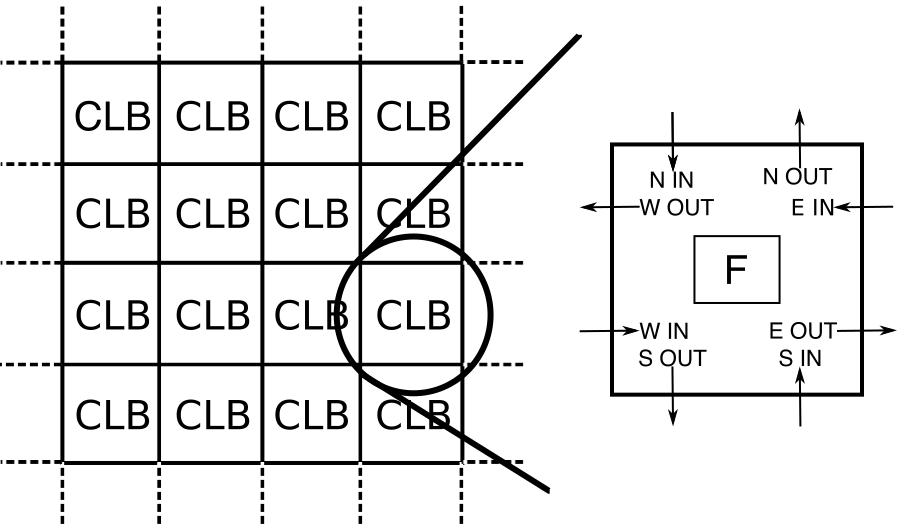
\includegraphics[width=.7\textwidth]{fpga.png}
\caption{FPGA architecture}
\label{fig:fpga}
\end{figure}

These immensely flexible circuits see wide use across industry. The most immediately
obvious example is
within firms developing more conventional integrated circuits who also ship accompanying
software. In these situations a team of engineers can develop software
while the hardware is developed in parallel, by using an FPGA loaded with a beta version
of chip. This avoids the many month wait times for a finished chip to be fabricated.
Recently FPGAs have seen a great deal of use as deep learning accelerators
\cite{Zhang:2015:OFA:2684746.2689060}; this is because FPGAs
configurations are cheaper to develop than ASIC hardware,
and see huge performance and power consumption benefits over more general purpose
hardware (GPGPUs for example). The flexibility also means iterative improvements
can be made to coincide with emerging research without the need to purchase new
hardware. Similarly, many industrial institutions require
bespoke hardware solutions to small-scale specific problems; suppose there is a
demand for a real time, high performance
pump controller which will only be used in a handful of locations. In these situations,
more often than not, ASIC
development is too expensive and not worth the narrow application setting. This demand has resulted in
the widespread use of FPGAs
in roles requiring an ASIC but without the market pressure to drive ASIC development
\cite{4267891}.
An application specific design can be built on an FPGA, while approaching peak performance and power
efficiency without massive development costs.
The military \cite{1346835} and aerospace \cite{henaut2009fpga} sectors use FPGAs extensively for these reasons along with
the built-in cryptographic and anti-tamper hardware obfuscation capabilities on
military-grade FPGAs.

\subsection{Genetic Algorithms}
The core of any genetic algorithm takes a randomly seeded population of binary strings
and applies
evolutionary pressure by performing a cycle of selection, crossover (an optional
step), and mutation
to move the population towards potential solutions to a given problem \cite{Goldberg:1989:GAS:534133}.
Beyond this there are many
variations, some of which will be explored in this thesis. The basic genetic algorithm is
outlined in Algorithm~\ref{alg:basic}.

\begin{algorithm}
	Randomly initialise a population $P$\\
	\While{evolving}{
		$Evaluate(P)$\\
		\While{New population $P'$ not full}{
			\eIf{Crossover occurs}{
				$p_1 \leftarrow Select(P)$\\
				$p_2 \leftarrow Select(P)$\\
				$i_1,i_2 \leftarrow Crossover(p_1,p_2)$\\
				Add $i_1$ and $i_2$ to $P'$
			}{
				$i \leftarrow Select(P)$\\
				Add $i$ to $P'$
			}
		}
		$P \leftarrow Mutate(P')$
	}
	\caption{Basic genetic algorithm}
	\label{alg:basic}
\end{algorithm}

An initial population is randomly generated and then
evaluated ($Evaluate(P)$). Evaluation provides each individual in the population with a score.
Members of a new population are generated by selecting members of the old population
at random, based on some selection mechanism (the most common schemes will be outlines
in Chapter~\ref{chap:technical}) and the scores each individual received. The individuals
selected in this manner have a single parent, some genetic algorithms also have a mechanism
by which an individual can have two parents; this is called crossover. Crossover has a
random chance of occurring, if it does, two individuals are selected from the old
population (via $Select(P)$), then from a random point in each parent's bitstring, the
parents swap
genetic material. This generates two new individuals, both are added to the
new population.
Finally, if an individual is made up of a bitstring of length $l$ and we have a mutation rate
of $m$, the $Mutate(P')$ function iterates over each bit in each individual, flipping the bit with
probability $\frac{m}{l}$. The new population $P'$ then replaces the old $P$, and the cycle continues.
These simple processes coalesce into a high performance robust search
procedure. Genetic algorithms are covered in more detail in Section~\ref{s:genetic}.

\subsection{Genetic Algorithms with an FPGA Configuration}
In a biology a genotype is an organism's DNA, and a phenotype is
the organism itself, the expression of the DNA. In the context of genetic algorithms,
the genotype is a binary string which is mapped onto a phenotype (in evolvable
hardware, often an FPGA configuration). When designing an evolvable hardware
system one must decide how to map from binary string to FPGA configuration.

Given a mapping from binary string to FPGA configuration and an FPGA test bed, one can
evaluate a population of bitstrings as the FPGA configuration to solve some digital
problem. This framework is at the core of evolutionary hardware. The bottleneck for physical evolvable
hardware is often the evaluation step, this involves converting each individual
to an FPGA configuration, uploading each in turn
to the FPGA, and extensively testing it. When each upload takes in the order of
multiple seconds the evaluation process can be laborious. To resolve this problem
many platforms simulate an FPGA until a design is chosen to be deployed, this reduces
training time aggressively, and is the direction this project has taken.

\section{Dynamic Problems}

A problem with evaluation critera which shifts over time is termed a dynamic problem.
Designing
evolutionary hardware robust to this set of problems is of considerable benefit as
dynamic problems span a class of practical but notoriously problematic challenges including
real-time optimisation, and fault tolerance.

\subsection{Hardware Faults}
Hardware faults are catastrophic for electronic devices. A relatively short life span is
mostly accepted, and is relatively benign in many areas; but when the cost of replacement is
extraordinarily high or the scale of the operation is large enough, there are huge benefits
to improving the fault tolerance of devices. An extreme example of the high cost of replacement
can be found with satellites, surveys of in-orbit satellites reveal that once deployed the
reliability of satalites drops aggressively, and despite the highest manufacturing standards,
after 15 years reliability drops to below
90\% \cite{CASTET20091718}. Be it due micrometeor impacts,
or the ionising effects of radiation, satellites are known to fail and a great deal of
work is expended improving their reliability. With the cost
of putting a satellite into orbit set in the millions of pounds, extending the lifespan
of such devices would have significant economic impact.

A little closer to home, data centres are vast structures contain thousands of servers.
Each of these has an 8\% probability of experiencing a failure each year
 \cite{Vishwanath:2010:CCC:1807128.1807161}.
Individually this is of no great concern, but when compounded across an entire data centre
server recovery and replacement becomes a primary concern for the management of
such an establishment.

One popular use of dynamic problems in evolutionary hardware is designed to breed
fault tolerance into a
design. This involves repeatedly turning on and off simulated faults in the FPGA during
evaluation in order to
create a design both robust to faults and not dependent on faults, as could happen if
only evaluated in a faulty system \cite{651463}. Another fault resilience
technique requires evaluating the configuration
against a fault-free FPGA and then combining the result with evaluation runs on FPGAs
simulating known frequent faults \cite{651463}\cite{Keymeulen2000}. These faults could include component
wear out, and manifest as blocked communications between CLBs or render the function
performed by a CLB inert. This extension of the fitness function (rather than
mid-execution fitness function modification) removes this approach from the domain of dynamic problems,
but it is worth noting as an alternate method to improve circuit reliability.

All of these methods require faults to be set before the genetic process begins, and can only be used to
develop evolvable hardware tolerant to specific faults. This requires a huge amount of knowledge
about the underlying hardware implementation and the frequency and severity of faults to generate
accurate fault models. This
is an important avenue of exploration but with evolvable hardware there is a missed
opportunity, with a system capable of quick iterative improvements, to work around
a problem as it occurs. This idea has been briefly explored in \cite{10.1007/3-540-61093-6_6}.

\subsection{Dynamic optimisation}
Another successful area of dynamic problems with evolutionary hardware involves
extending the evaluation function when a perfect solution has been found \cite{785435}. For example,
one could successfully evolve an audio filter and then incorporate a measure of ``smallness"
into the fitness. This would add evolutionary pressure to not only be correct, but also
use as little of the FPGA resources as possible.

Little work has been done exploring the reaction of evolvable hardware to tackling
related-but-not-identical problems (addition and subtraction, for example), and observing
the effect of varying
the relative benefits for correct answers for either, on the performance of the circuit for each problem.
Information in this domain could
drive development of systems capable of dynamically optimising in real-time
under shifting conditions.

\section{Project Aims}

The broad aim of this project is to develop an improved evolvable hardware
platform capable of effectively addressing dynamic problems. More specifically:
\begin{itemize}
	\item Apply the genetic algorithm from \cite{10.1007/3-540-63173-9_61} to
		the binary arithmetic problem.
	\item Combine state of the art genetic algorithms to improve
		evolvable hardware performance for binary arithmetic.
	\item Explore the application of evolvable hardware to dynamic
		problems, including FPGA faults and weighted binary arithmetic.
	\item Develop a specialised FPGA simulator to act as the evaluation
		back end for the genetic algorithm.
	\item Study and improve the scaling performance of evolvable hardware.
\end{itemize}

\section{Project Challenges}
The project is not without challenges:
\begin{itemize}
	\item There are few ways to evaluate individuals and population health beyond how
		correct they are, so understanding why a system works or does not work may
		be difficult.
	\item The issue of scaling will slow development of anything other than
		trivial problems (2-bit addition and subtraction).
	\item FPGA configurations for a variety of problems investigated here are very fragile, in the
		context of evolution. Frequent mutations could be disastrous.
	\item More so than in many evolutionary contexts the prospect of evolutionary dead ends
		and dominating local optima will need to be addressed.
\end{itemize}


% -----------------------------------------------------------------------------

\chapter{Technical Background}
\label{chap:technical}

{\bf \color{red}A compulsory chapter,     of roughly $10$ pages} 
\vspace{1cm} 

{
	\color{red}
\noindent
This chapter is intended to describe the technical basis on which execution
of the project depends.  The goal is to provide a detailed explanation of
the specific problem at hand, and existing work that is relevant (e.g., an
existing algorithm that you use, alternative solutions proposed, supporting
technologies).

Per the same advice in the handbook, note there is a subtly difference from
this and a full-blown literature review (or survey).  The latter might try
to capture and organise (e.g., categorise somehow) {\em all} related work,
potentially offering meta-analysis, whereas here the goal is simple to
ensure the dissertation is self-contained.  Put another way, after reading
this chapter a non-expert reader should have obtained enough background to
understand what {\em you} have done (by reading subsequent sections), then
accurately assess your work.  You might view an additional goal as giving
the reader confidence that you are able to absorb, understand and clearly
communicate highly technical material.
}

This chapter provides the technical background to the project and discusses
the relevant existing work.

\section{Genetic Algorithms}
Genetic algorithms grew from a branch of engineering which takes influence from
nature. By applying Darwinian evolutionary theory to a population of binary strings
they developed
a robust directed nondeterministic procedure to navigate search spaces with noncontinuous
fitness. These search spaces are not well suited to conventional search methods,
such as innumerated bruteforce or heuristic driven methods like A* search,
and previously were only navigable by simple hill-climbers, random walks, or bruteforce search,
and genetic algorithms provide a good general method to approach problems where
such little information is known about a space of solutions.
David Goldberg's book {\em Genetic Algorithms: In Search Optimisation \& Machine
Learning} \cite{Goldberg:1989:GAS:534133} contains a good summary of the knowledge
of genetic algorithms as it stood in the early 1990s.
The genetic algorithm as presented by Goldberg consists
of a repeated cycle of reproduction, crossover, and mutation; and operates on a
population of randomly seeded binary strings.

\paragraph{Reproduction}
is the mechanism by which a new population is generated. Given a fitness function
$f$ providing a measure of the quality of an individual, each member of the
population is evaluated and
assigned a score. To improve the fitness across the entire population some form
of Darwinian selection is used so that the probability of an individual
reproducing is higher for individuals with better fitness.
One such commonly chosen selection mechanism is roulette wheel (stochastic) selection.
For each individual $x$, in a population of size $n$, with fitness function $f$,
the probability of $x$ producing offspring with roulette wheel
selection is given by equation~\ref{eq:roulette}. After the reproduction
stage a new population has been created, sampled from the old.

\begin{equation}
	P(x) = \frac{f(x)}{\sum_{i=0}^{n}f(x_{i})}
	\label{eq:roulette}
\end{equation}

\paragraph{Crossover} is an optional part of the core genetic algorithm definition
provided by Goldberg \cite{Goldberg:1989:GAS:534133}. It
allows two strings to act as parents and share genetic material for an individual
in the new generation. Given a crossover probability, each slot in the new population
has a chance to be filled by an individual in the previous generation selected
by the given selection mechanism. If crossover is selected as the means to
fill a position in the new population two parents are selected by the genetic
algorithm selection mechanism,
, a number $k$,
is selected such that $1 \leq k \leq l$, where $l$ is the population string length.
Both individuals, then swap every bit from position $k$ onwards.

\paragraph{Mutation}
occurs after reproduction and crossover. Given a population of strings each of length
$l$, and the number of mutations expected per individual, $m$, each bit of each string
is flipped with probability $\frac{m}{l}$.

\paragraph{}
These relatively simple mechanisms provide the non-deterministic but focussed,
and surprisingly robust search procedure capable of addressing a problem when
little is known about the search space and systematically forming an answer is
unfeasible.

An interesting tangential application of FPGA technology to evolutionary algorithms comes as
a physical evolution hardware accelerator \cite{1377261}, which uses the flexibility from the
FPGA to allow incremental runtime hardware changes which allow the hardware realisation of
functions which would otherwise be impossible to construct directly in hardware, to the
need for fluid function reconfigurability.
This highlights the opportunity for aggressively efficient evolvable hardware
systems.

\subsection{Selection Mechanisms}

Goldberg et al. offer a comparison of common selection schemes for use in genetic
algorithm reproduction \cite{GOLDBERG199169}. They compared proportionate
selection, rank based selection, and tournament selection, amongst others.

\paragraph{Proportionate selection} is any selection scheme in which the probability
of an individual being selected as a parent is proportional to their fitness score.
This includes roulette wheel selection.

\paragraph{Rank selection} orders each member of a population by their
fitness. Then the probability of each individual being selected as
parent is proportional to their position in the ranking. This serves as
a way to "flatten" out the selection curve, and reduces the influence of
a huge spread of individual fitness. Commonly a linear ranking is chosen,
in this the most fit individual is twice as likely to be selected
as a parent as the individual with median fitness.

\paragraph{Tournament selection} is a type of proportionate selection,
which operates by randomly selecting a subset of the
population and the best individual from this set is chosen for further genetic
processing. Tournaments can be as small as consisting of 2 individuals, or much
larger.

\paragraph{}
There are key differences between these selection mechanisms which influences
the descision to incorporate them into an evolvable hardware platform. Proportionate
selection discriminates heavily by the fitness of individuals. Rank based
discriminates less and cares more about who is better (rather than by how
much they are better). Tournament selection discriminates intensely within a given
tournament but the selection process to assemble the tournament is uniformally
random, so depending on the tournament size this can be highly discriminatory
(large tournament size) or minimally descriminatory (small tournament size).
At certain tournament sizes tournament selection performs similarly to roulette
wheel selection.
For evolvable hardware proportionate selection sees little use due to the range
of fitness values often associated with members of the population, rank and
tournament selection is frequently used.

\subsection{The Fitness Function}

\begin{equation}
	f(x) = \sum_{i=1}^{z} w_i f_i(x)
	\label{equ:multi-obj}
\end{equation}

By extending the fitness function to a weighted linear combination of a function
measuring correctness (the original fitness function)
and any other measurements we can deploy evolutionary pressure to optimise for
additional parameters \cite{deJong:2001:RBP:2955239.2955241}. For an individual
$x$, a set of functions measuring distinct desirable aspects of individual
$\{f_1,f_2,\ldots,f_z\}$, and a set of weightings associated with each function
$\{w_1,w_2,\ldots,w_z\}$ the new fitness function $f(x)$, is given by
Equation~\ref{equ:multi-obj}.

This technique has been used to expand the success criteria for a evolvable hardware configuration
to create smaller, or more fault resistant hardware designs.

\subsection{Coevolution}

Coevolution refers to the practice of evolving two populations in tandem, this can
act as a way to divide labour (two populations solving different parts of a problem)
 \cite{Potter:2000:CCA:1108888.1108890},
or as adversaries (one population of problem proposers and another of problem solvers).
The former is used to improve the scalability of evolvable hardware to naturally
decompose the problem into subproblems.
The latter is often likened to a host/parasite or prey/predator relationship.
The framework for a coevolutionary system is only a slight extension to the
generic genetic algorithm outlined previously. In a competitive system, $P_s$ is a randomly
seeded population of problem solvers, and $P_p$ is a randomly seeded population
of problem proposers; where each individual is represented by a bitstring of
appropriate length. The fitness function of one population is inexorably tied to
the fitness function of the other.
When evaluating, each problem solver $p_s \in P_s$ is randomly associated
a problem proposer $p_p \in P_p$, and is scored based on how many problems proposed by
$p_p$ that are correctly solved. $p_p$ is scored based on how many problems
are incorrectly solved. Once each individual is scored the genetic process continues as expected,
with independent reproduction, crossover, and mutation for each population.

The evolutionary pressure on the problem proposers pushes them to be as difficult
to solve as possible, therefore emphasising problems the population of solvers
find difficult. This proves a highly effective distinguishing tool, and produces
problem proposers which create hard problems specifically tailored to the population
of problem solvers \cite{HILLIS1990228}.

Extending the parallel with nature, one can modify the virulence of the parasitic
coevolutionary population. Virulence is a measure of the hostility of the aggressor.
Malaria is a highly virulent virus, often killing it's host; the evolutionary
process which drove it's development encourages causing maximum harm to the target.
An example a of virus with a low virulence is the common cold, it gains nothing from
killing the host, it wants the host to survive and spread the virus; this means
there is evolutionary pressure discouraging a maximal virulence.

In some settings a population of highly virulent problem proposers develop to be much more
aggressive than the solvers can handle, meaning no solver ever manages to
successfully solve any problem, even if it could have solved some easy ones.
When individuals can no longer
differentiate themselves and push the population up the evolutionary ladder,
the coevolved populations are said to have disengaged.
By modifying the fitness function Bullock et al. \cite{6790490}
discouraged maximally
virulent parasites. This encourages populations to stay engaged, and improved the
quality of discovered solutions.

\section{Evolvable Hardware}

\subsection{Theory}
The foundational work in evolveable hardware is summarised by T. Higuchi et al. in their
paper {\em Evolvable Hardware with Genetic Learning} \cite{541893}. They describe
the flexibility of FPGA devices and how this can be exploited by genetic algorithms
by treating the bitstring used by the hardware for calibration as the genetic material
to be evolved. They also describe the fitness function as the total number of correct
output bits read off the hardware for all possible inputs. They succeed in evolving multiplexors and
counters but highlight a limitation of the direct evolution of the FPGA calibration
bitstring; only a subset of the bitstring include bits relevant to the function
of a specific region of the hardware, some bits were redundant, act as checksums, or
perform routine non-optional calibration. This increase in the amount of genetic
material expands the search space and extends the time required for the genetic algorithm to find a solution.
Using the proposed framework they evolve an image pattern recognition system,
and a welding robot controller which takes sensor information and traces a ditch.

They highlight the need to abstract from gate level evolution to improve the
execution times of the genetic algorithm and present function level evolution
as a solution. This involves replacing gates (AND, OR, NOT, etc.) with functions
(adder, subtracter, etc.) as the atomic evolutionary components. Figure~\ref{fig:mapping}
outlines the principal, instead of evolving the configuration bitstring directly
a mapping is defined which translates a binary string into a collection of
logic gates. This logic structure can then be synthesised into an FPGA configuration
bitstring and is uploaded to the device.

\begin{figure}
	\centering
	\begin{subfigure}[ht]{0.4\textwidth}
		\centering
		\ldots 0010101010100010101011 \ldots
	\end{subfigure}
	~
	\begin{subfigure}[ht]{0.1\textwidth}
		$\rightarrow$
	\end{subfigure}
	~
	\begin{subfigure}[ht]{0.4\textwidth}
		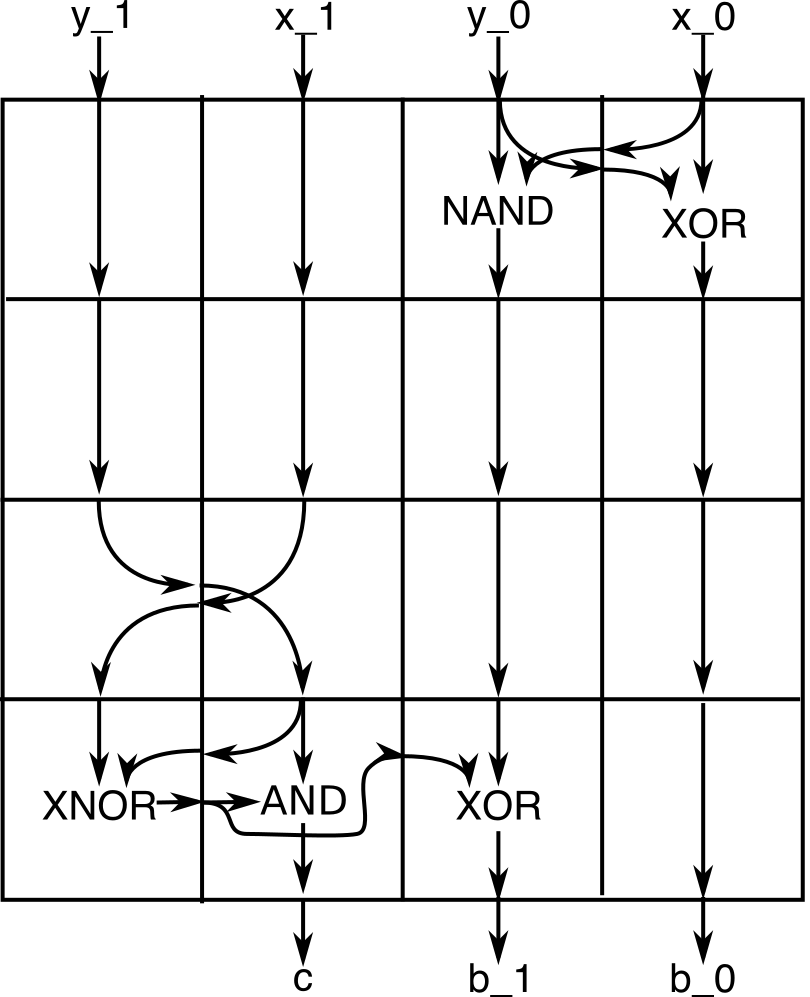
\includegraphics[width=\textwidth]{evolved_adder}
	\end{subfigure}
	\caption{For gate-level evolution a mapping has to be devised from bitstring to logic structure.}
	\label{fig:mapping}
\end{figure}

The capacity for evolutionary hardware to come up with bespoke and novel solutions
was explored by Adrian Thompson \cite{10.1007/3-540-63173-9_61}. A genetic algorithm
operated on a 10x10 grid of cells in the top corner of an FPGA, the aim was to evolve
a circuit capable of differentiating a high frequency input signal (10kHz) and a
low frequency input signal (1kHz). The output signal should read "high" (+5V) for one frequency
and "low" (0v) for the other. This was a truly bespoke application of evolutionary
hardware as the region exposed to the genetic algorithm had no access to any
hardware capable of timing; the differentiation task was one which the hardware
conventionally would not be able to do.

The algorithm driving evolution was standard in many respects; with a population size of 50,
the most fit individual was copied verbatim into the next generation (a mechanism
called {\em elitism}), and linear rank-based selection (where the fittest
individual had a probability of selection double that of the median individual)
was used for the remaining members of the population. The probability of (single-point)
crossover occurring was 0.7 and the expected number of mutations per individual
(except the individual copied over via elitism) was 2.7. These values are in
accordance with existing research and were arrived at after domain specific
experimentation.

The 100 cell area was encoded as a string of 1800 bits. Each cell was defined
left-to-right row by row. The fitness evaluation was conducted on physical hardware
(many EHW schemes use simulations to improve training time), a series of test frequencies
were fed into the device and a single cell's output was read. The fitness of a configuration
was defined as the difference between the average output for each of the two input frequencies
(multiplied by a constant to avoid otherwise inescapable local optimum), therefore the larger
the distinction the more fit the configuration was deemed. Without the constants in the
fitness function the genetic algorithm directly connected the input and output of
the circuit through the FPGA creating a useless configuration which performed
well enough to discourage any further exploration.

After 3500 generations of evolution the genetic algorithm produced a specification
capable of distinguishing the two input signals cleanly. This is behaviour beyond
what the hardware was designed for and demonstrates the power of evolvable hardware. One of the
interesting things to come from Thompsons work was the demonstration that genetic
algorithms happily exploit undefined and strange behaviour on-chip, such as feedback
loops and more strangely; unconnected circuitry. The successful
individual's schematic was pruned of any circuitry which should not influence the
output (a direct path could not be traced from the input to the output via that route),
and the fitness of what remained {\em dropped}. This reduction in quality was attributed
to strange undefined chip behaviour, unwhittingly exploited by the genetic algorithm.
FPGA cells exerted subtle influence over neighbouring cells despite the absence of any explicit
connection.
The search procedure took 2-3 weeks
due to each evaluation taking up to 5 seconds.

By extending the fitness function we can apply evolutionary pressure to configurations
to nurture more than just correctness.
One of the first uses of multi-objective fitness function in evolvable hardware was
to reduce the size of the circuit \cite{785435}. Once a correct solution has been evolved the
fitness function shifts to a linear combination of correct output bits and
the number of cells innactive. This paper also introduced a mechanism for evolving the size
and shape of the underlying fabric in parallel to conventional evolvable hardware
evolution, this allows for a system to define
how large it should be.
Both multi-objective fitness functions and evolved circuit structure
apply evolutionary pressure to improving the quality of evolutionary hardware
beyond simple performance accuracy.

An alternative substrate for evolvable hardware to FPGAs comes in the form of field
programmable transistor arrays (FPTAs) \cite{869347}. These offer similar functionality
to FPGAs, but where FPGAs allow gate-level flexibility, FPTAs allow a user to specify
the placement and configuration of transistors. Evolutionary hardware operating on this
level is subject to worse scaling issues than gate-level evolvable hardware, but has a
great deal more flexibility.

One of the largest problems with evolvable hardware is how the system scales as the
circuit function increases. The poor scaling of the genetic algorithm is due to two
features; the larger circuit size required (and the consequently larger genetic material),
and the larger number of test-cases in the evaluation function. One way to combat this
involves decomposing the problem into subsystems \cite{10.1007/978-3-540-46239-2_5}.
This reduced granularity shrinks the search space of solutions and improves search
performance at the cost of the flexibility to construct novel circuitry.

A similar method proposed by J. Torrensen suggests allowing the evolutionary
process itself to subdivide the process, increased complexity evolution \cite{Torresen2002}. The area
of an FPGA is divided into subsets of cells and the function of each of these
subsets is decided manually or by the evolutionary process.
The first system, dubbed ``partitioned training vectors" involves feeding the
complete input information individually to each subset, but only reading off
a subset of the output bits from each region of cells. In this way each subset
can distinguish a few answers perfectly and the other input combinations are
identified by another group of cells.
A parallel is drawn
with artificial neural nets where evolution is applied to the connections between
these subsets, and each subset evolves it's functionality locally. To demonstrate
the efficiency of such a system using the vector approach a character detection system was evolved, capable
of classifying images of letters of size 5 by 6 pixels, the number of generations
required to train the classifier dropped substantially as the number of allowed subsystems
increased. More success was found applying this technique to a prosthetic hand controller
which achieved better performance than the artificial neural net equivalent.
A similar decomposition strategy has been proposed in \cite{1703646}, with the
aim of reducing the number of generations needed to sufficiently explore the search
space by automating the division of problems when the genetic algorithm appears to
be making no progress and is stalling.

These methods all deal with reducing the search space or dividing the problem into
more manageable workloads. The problem remains with the scaling inefficiency in
regards to the number of test cases to be applied to a circuit during evaluation.

This other, less explored facet of the scaling issues appears in the form of the number of
evaluations required to calculate the fitness function. For evolved circuitry
with $n$ input bits, the fitness function requires $O(2^{n})$ time to evaluate;
for example, a 2-bit adder requires evaluation against all 16 ($2^{2 \cdot 2}$) possible combinations
of 2 2-bit numbers, whereas for a 3-bit adder this value grows to 64 ($2^{2 \cdot 3}$).
For practical evolution of larger circuits this requires some careful thought.

A novel approach to shrinking the search spaces involves using compression
techniques to reduce the size of the genetic material. \cite{1508485} uses
Lempel-Ziv compression to limit the genome complexity and suggest directing
research into evolvable hardware scaling to considering only ``active" areas
of the genetic material and limit the search space to only include meaningful
distinctions between circuits.

\subsection{Application}

Part of the charm of evolutionary hardware is it's vast capacity for strange
solutions
to problems. The nature of a simple fitness function driving the evolutionary
process means that any point in the search space which performs perfectly is
equally weighted as any other point in the search space.

Nowhere is this more apparent than with the antennas featured on NASA's ST5 mission
which were designed by genetic algorithms \cite{Antenna}. Although
this is a slight departure from the circuit design applications mentioned thus
far it is a fantastic example of the strengths of evolution derived design.
Traditional (human-driven) antenna design is a laborious process requiring
seasoned professionals with a great deal of experience in the area. By creating
a fitness function which outlined the design requirements of the device, and
tuning a suitable genetic algorithm, huge portions of the design process can
be automated.

Figure~\ref{fig:antenna} features the evolved antenna design which
saw use in space. Clearly it is a novel design, looking like an art piece
more at home in the Tate Modern than a piece of space-grade equipment, and such
designs are typical of evolved systems. The antenna performed successfully
throughout the operational lifetime of the spacecraft. This avenue of design
provided completely fresh ideas, unburdened by the prejudice of previous
success. The antenna achieved a larger range of detection angles than the
hand designed counterpart and required only 3 person-months of work to set up and
monitor the evolutionary process rather than the 5 person-months of work which
would otherwise be required.

\begin{figure}
	\centering
	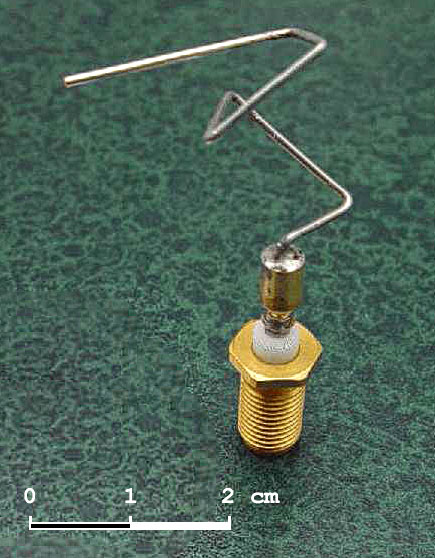
\includegraphics[height=5cm]{NASA_antenna.jpg}
	\caption{NASA evolved antenna \cite{Antenna}}
	\label{fig:antenna}
\end{figure}

The list of evolutionary hardware successes in digital ciruits is long \cite{Sekanina};
from logic circuit synthesis \cite{Vasicek2011} to high bandwidth image filter
evolution \cite{10.1007/3-540-46004-7_26}\cite{HybridFilter}.
Using tournament selection and elitism T. Higuchi et al.
developed a custom evolvable hardware chip for use in telecomunications and robots \cite{HiguchiRW},
claiming successful evolution of robot controllers and ciruits performing lossless image
compression outperforming existing standards. All this was performed on off
the shelf components designed to accelerate the evolvable hardware process
for gate-level evolution \cite{HiguchiRW}. A similar success story with hardware
designed for evolution takes the form of a prosthetic hand controller with
a training time of only 10 minutes to adapt to a new user \cite{Kajitani1999AnEH}.

In the name of robustness, adaptability and complexity, POEtic tissue
\cite{Tyrrell:2003:PTI:1766731.1766747} is
an effort to build an extended evolvable hardware platform inspired by
earilier work on phylogenesis (analysis of the evolution individuals and species),
ontogenesis (development of single-molecular organisms), and epigenesis
(the learning over an idividuals lifespan) \cite{10.1007/3-540-63173-9_37}.
These three traits inspire the genotype, mapping, and phenotype layer of the
hardware system proposed. This system would act as an evolutionary hardware
specific replacement for current FPGA systems.

Adding to the literature regarding the evolutionary scaling issue specifically
in the domain of evolvable hardware
Modular Evolvable Hardware (MEH) \cite{1299561} performs functional decomposition
of the overall hardware requirements and then individual module evolution.

\subsection{Arithmetic Circuits}

Binary arithmatic has seen some use as a benchmarking problem for evolvable systems.
The most common applications of genetic algorithms within the hardware space
are as learning robot/prosthetics controllers or fast image filters, however
in \cite{Miller_multiple-valuedcombinational} Kalganova et al. demonstrate the
capacity for evolvable hardware to generate 1-bit addition circuits. These
circuits are capable of adding upto 3 different variables and provide a carry-out
bit of a full-adder.

Successful evolution of robust 2-bit addition was achived by Miller et al. through
the deployment of tournament selection \cite{TournamentAdder}. This was evolved
in the presence of an imperfect fitness function and used the adjustable selection
pressure of tournament selection to develop a fine-tuned genetic algorithm tailor
made for various noise levels.

\section{Dynamic Problems}

Dynamic problems are challenges which change over time. These can take many
forms, from scheduling \cite{LIN1997AGA}, to fault mitigation, and optimisation problems
\cite{Branke2003}. The vast majority of evolutionary computing research focusses on
static problems, but the dynamic varient are more indicative of real problems.
In \cite{LIN1997AGA} Lin et al. develop a genetic algorithm
which schedules continously arriving jobs. A series of dynamic qualities, including
timing information job importance fed into a multi-objective fitness function. This
approach improved over current deterministic job scheduling schemes. \cite{Branke2003}
details the use of distinct sub-populations in a multi-population structure to
improve diversity and better tackle the bredth of a dynamic problem.

\subsection{Fault Tolerance}

A dynamic problem specifically in the domain of evolvable hardware is fault
tolerance.
In hardware design, fault tolerance is defined as a systems capacity to
remain functional despite component failure. This is usually in reference to
post-fabrication faults which affect can effect chip yields, but evolutionary
hardware also looks extensively into faults which occur some way into the
operational lifespan of a product; this can be component failures do to environmental
conditions or an aging device.

Genetic algorithms by their nature produce designs which are resilient in the face
of change \cite{10.1007/3-540-46406-9_14}\cite{651463}. If a solution is perticularly fragile a
simple single mutation could cripple its performance, the probability that an individual
has successful offspring is therefore directly tied to the probability an individuals is
able to perform well
despite being subjected to random mutations. More fragile designs are often
mutated into obscurity whereas ones with
natural fault tolerance endure. Over time this tendancy to maintain a population
of individuals capable of surviving minor changes leads to a naturally fault tolerant
solution.
Amplifying the effects of this subtle pressure towards fault
tolerant design is a mainstay of applied evolutionary hardware research.

In \cite{10.1007/3-540-61093-6_6} a robot welding controller designed to trace
ditches comes equiped with an evolvable hardware backup system which is activated
should a hardware fault be detected. Controllers such as these conventionally use
FPGAs anyway \cite{4267891}; the economy of bespoke high-performance industrial requirements
often make FPGAs the best choice (as detailed in Subsection~\ref{ss:FPGAs}). Because of
this there is a prime opportunity to deploy evolvable hardware to recover from
a fault which would otherwise require a compelete hardware overhaul. \cite{10.1007/3-540-61093-6_6}
succesfully demonstrate such capacity.

Along with Adrian Thompson's genetic algorithm exploting undefined chip behaviour
\cite{10.1007/3-540-63173-9_61}, in another paper Thompson also notes that evolveable
hardware has designed
systems which rely on undefined temperature sensitive component behaviours
\cite{Thompson:1998:ADR:645508.656773}. In order to breed solutions capable
of functioning on different chips and in a broad array of conditions an extended
fitness function
was developed to apply selection pressure to temperature robustness qualities.
This fitness function repeated the evaluation step on a series of different FPGAs
at different temperatures and then combined the results.

One of the potential problems with fitness function driven exploration comes in
the form of environment specific effects. Somefolk et al. explored the problem
where the evolutionary process honed in to a solution which exploited temperature
sensitive behaviours of a chip \cite{10.1007/BFb0057603}.

By defining a list of the faults a device is expected to encounter during it's
lifespan one can design a fitness function which tests a given circuit under
normal conditions and faulty conditions \cite{651463}\cite{Keymeulen2000}. This technique applies explicit
evolutionary pressure to find designs which can tolerate a specific set of
known and understood faults. Alongside the proposed fitness driven fault mitigation
approach \cite{Keymeulen2000} introduces an alternative mechanism which takes the
highest performing individual in a fault-free system and explores the performance
of mutants generated from it in a fault environment, this emphasises the natural
fault tolerant properties of genetic algorithms. In some situations the mutants
could not recover from the injected fault, in these cases the genetic algorithm
was to restart and continue searching through the design space under the conditions
of the fault.

Using a conventional genetic algorithm, along with tournament selection, and elitism
J. Lohn et al. demonstrate the capacity
of evolvable hardware to reduce the impact of "stuck at zero" faults \cite{10.1007/3-540-36553-2_5}. They
conducted their experiments on a simulated FPGA, attempting to evolve a quadrature
decoder, a device which indicates
the direction of rotation of a wheel. The system was evolved in the presence
of the fault and was capable of operating perfectly despite it.

Despite major advances in chip fabrication technology, due to transistors
approaching the attomic scale, post-fab faults are a major issue. Walker et al.
demonstrate the capacity for genetic algorithms to design hardware which would
improve fabrication yeilds \cite{10.1007/978-3-540-85857-7_27}. The structures
they successfully evolve prove highly tolerant to variations in fabrication process
and they demonstrate the possibility to improve the success rate of chip manufacture
through deployment of evolutionary hardware design.

The space industry naturally wants to emphasise longevity in their design goals,
this was a clear desire with the NASA's CT5 mission, and as previously mentioned
the genetic algorithm devised antenna performed to the highest standards until the
end of the missions lifespan \cite{Antenna}.

Circuitry hosted in space is subject to a breadth of extreme conditions; temperature
drifts, radiation, and poor serviceability to name a few. Radiation is a particular
issue, bombarding electronics with electrons and protons causes huge damage.
The space industry has traditionally used radiation-hard materials to achieve
radiation resistance. These materials resist the ionising effects of radiation
and reduce the probability of radiation-induced silicon faults. These materials
are expensive and definitely not the only way to create long-life deep space
electronics. Sotica et al. propose using genetic algorithms to drive
in-situ hardware reconfiguration to bypass faulty areas \cite{1331112}. Experiments
were performed on an FTPA with evolution controlled by an external stand-alone
board-level evolvable system (SABLES) capable of performing an evaluation in 2ms.
In experiments bombarding the chip with upto 350krad the system was usually able
to recover functionality, and there were significant performance improvements over
the unevolved comparison chip.

In \cite{8046381} a brushless DC motor control circuit with built in hardware capable of executing
a genetic algorithm was shown to be capable of self-repairing damage to upto 27.8\%
of the hardware resource. Their system requires the complete shut down of the motor while
evolution finds an alternative control circuit configuration.

Fault tolerance in conventional hardware design requires redundancy in some
form. Predictive preemptive instruction rescheduling on a different processor
core \cite{Soman} uses multi-core redundancy to mitigate the cost of faulty instruction
execution. Cross-core redundancy is used by core salvaging \cite{Powell} which shares execution
pipeline resources between cores, in order to reroute execution pipelines
around faulty components. This is similar in principal to StageWeb \cite{StageWeb}, which also
features pipeline rerouting but with an emphasis in scaling flexibility.

This is a very different approach to evolvable hardware centric fault
tolerance which exploits flexibility. Many of the aforementioned modern
fault techniques do little to improve the performance of faulty architectural
processor components and rely on the ability to route around them.

The bulk of evolvable hardware research addresses ``toy problems", and is a long
way from being able to compete against conventional fault tolerant design
techniques \cite{4291951}. But there have been promising results and unprecidented
ability to design circuit structures with uncanny fault suvivability properties.


% -----------------------------------------------------------------------------

\chapter{Project Execution}
\label{chap:execution}

{\bf \color{red}A topic-specific chapter, of roughly $15$ pages} 
\vspace{1cm} 

{
\color{red}

This chapter is intended to describe what you did: the goal is to explain
the main activity or activities, of any type, which constituted your work
during the project.  The content is highly topic-specific, but for many
projects it will make sense to split the chapter into two sections: one
will discuss the design of something (e.g., some hardware or software, or
an algorithm, or experiment), including any rationale or decisions made,
and the other will discuss how this design was realised via some form of
implementation.

This is, of course, far from ideal for {\em many} project topics.  Some
situations which clearly require a different approach include:

\begin{itemize}
\item In a project where asymptotic analysis of some algorithm is the goal,
      there is no real ``design and implementation'' in a traditional sense
      even though the activity of analysis is clearly within the remit of
      this chapter.
\item In a project where analysis of some results is as major, or a more
      major goal than the implementation that produced them, it might be
      sensible to merge this chapter with the next one: the main activity
      is such that discussion of the results cannot be viewed separately.
\end{itemize}

\noindent
Note that it is common to include evidence of ``best practice'' project
management (e.g., use of version control, choice of programming language
and so on).  Rather than simply a rote list, make sure any such content
is useful and/or informative in some way: for example, if there was a
decision to be made then explain the trade-offs and implications
involved.
}

The core of this project involves building a flexible evolvable hardware
platform upon which novel genetic algorithm can design solutions which can be
evaluated in a narrow context. Due to the high demands of an iterative
design cycle, reducing the evaluation time within the genetic algorithm is
at the forefront of the design process; to this end a simulated FPGA is used
to simplify development and improve the speed of evolutionary training.

A single problem has to be chosen to which we will tailor the genetic process.

\section{Project Management}
The sourcecode is hosted online at \url{https://github.com/AlexDalt/MalleableHardwareAdder},
it's written in C to maximise training performance and Git was used for version control.
Regular supervisor meetings ensured the project stayed focussed. The aims
of the project are reduced to evaluating various performance metrics of
different and new evolvable hardware processes.

\section{Design}
The high level design choices have been made to improve development time
and discern insights into evolutionary hardware with dynamic problems and
the scaling issues involved. The system should be flexible so parameters can
be altered between searches and infomation
about the population performance should be offered as the genetic algorithm runs.

\subsection{Phenotype to Genotype Mapping}
The mapping from binary string to FPGA configuration is one of the first design
choices to be made. The simulated FPGA will be of configurable width and height, and each
cell will operate as described in \cite{10.1007/3-540-63173-9_61} and Figure~
\ref{fig:fpga}. Each cell takes
input from each of it's neighbours, performs a binary function $F$ on chosen input(s)
and sends distinct configurable outputs to each of it's neighbours. The binary
function $F$ or any of the inputs can be sent to any of the outputs.

To fully describe the operation of a cell a 15-bit binary string was chosen.
This is arranged in memory as 2 bytes per cell, of which one bit is unused.
The least significant byte defines all the outputs, 2 bits per neighbour
(from least significant bits to most significant bits: north, east, south,
and west), where a 0 is defined as a direct mapping from the northern input
to that output, a 1 means the eastern input is used, 2 the southern, and 3
western.  A description of
the complete string can be found in Figure~\ref{fig:bin}. In this example
the cell performs an XOR operation on the inputs coming from the cells to
the north and south. The southern input is mapped to the eastern output,
and the norther input is mapped to the western output. Both the northern
and southern outputs send the output of the XOR operation as under my
scheme
an output cannot be mapped to it's input, in the situation that the
number associated with an output refers to the input coming from the same
direction the function $F$ is used as input instead. As the northen output
is specified as 00 (NORTH) and the southern input is specified as 10 (SOUTH)
they both recieve the output of the function.

The most significant byte describes the function $F$. The low 2 bits describe
the first input (00 $\rightarrow$ north, 01 $\rightarrow$ south, 10
$\rightarrow$ east, 10 $\rightarrow$ west), the next 2 bits describe the second
input in the same manner, and the next 3 bits describe the operation performed
(000 $\rightarrow$ OFF, 001 $\rightarrow$ NOT, 010 $\rightarrow$ OR, 011 $\rightarrow$
AND, 100 $\rightarrow$ NAND, 101 $\rightarrow$ NOR, 110 $\rightarrow$ XOR, 111
$\rightarrow$ XNOR).

\begin{figure}
	\centering
	\begin{subfigure}[ht]{0.45\textwidth}
	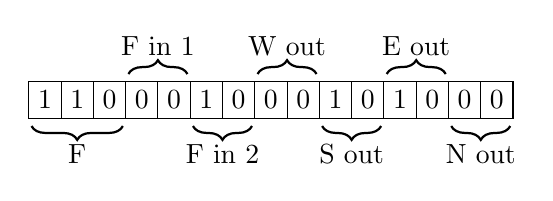
\begin{tikzpicture}[
node distance=0pt,
 start chain = A going right,
    X/.style = {rectangle, draw,% styles of nodes in string (chain)
                minimum width=2ex, minimum height=3ex,
                outer sep=0pt, on chain},
    B/.style = {decorate,
                decoration={brace, amplitude=5pt,
                pre=moveto,pre length=1pt,post=moveto,post length=1pt,
                raise=1mm,
                            #1}, % for mirroring of brace, if necessary
                thick},
    B/.default=mirror, % by default braces are mirrored
                        ]
\foreach \i in {1,1,0,0,0,1,0,0,
                0,1,0,1,0,0,0}% <-- content of nodes
    \node[X] {\i};
\draw[B] ( A-1.south west) -- node[below=2mm] {F} ( A-3.south east);
\draw[B=] ( A-4.north west) -- node[above=2mm] {F in 1} ( A-5.north east);
\draw[B] ( A-6.south west) -- node[below=2mm] {F in 2} ( A-7.south east);
\draw[B=] ( A-8.north west) -- node[above=2mm] {W out} ( A-9.north east);
\draw[B] ( A-10.south west) -- node[below=2mm] {S out} ( A-11.south east);
\draw[B=] ( A-12.north west) -- node[above=2mm] {E out} ( A-13.north east);
\draw[B] ( A-14.south west) -- node[below=2mm] {N out} ( A-15.south east);
    \end{tikzpicture}
	\end{subfigure}
	~
	\begin{subfigure}[ht]{0.25\textwidth}
		\centering
		\begin{tabular}{cc}
		\toprule
		Direction & Encoding \\
		\midrule
		NORTH & 00 \\
		EAST & 01 \\
		SOUTH & 10 \\
		WEST & 11 \\
		\bottomrule
		\end{tabular}
	\end{subfigure}
	~
	\begin{subfigure}[ht]{0.25\textwidth}
		\centering
		\begin{tabular}{cc}
		\toprule
		Function & Encoding \\
		\midrule
		OFF & 000 \\
		NOT & 001 \\
		OR & 010 \\
		AND & 011 \\
		NAND & 100 \\
		NOR & 101 \\
		XOR & 110 \\
		XNOR & 111 \\
		\bottomrule
		\end{tabular}
	\end{subfigure}

	\caption{Genetic representation for a single FPGA cell}
	\label{fig:bin}
\end{figure}

Cells are defined from left to right, top to bottom on the FPGA. Therefore the
binary strign required to describe an FPGA of width $w$ and height $h$ is $2wh$
bytes long.

This mapping was chosen because it is loosely in line with the number of bits
required by \cite{10.1007/3-540-63173-9_61} and it allows concise expression of
the FPGA. The order in which cells are defined also follows
\cite{10.1007/3-540-63173-9_61}, and means any crossover occurring tends to keep
the horizontal sections consistent with each other.

\subsection{Problem Choice}

The choice of problem is a key component in designing and configuring the genetic
algorithm to tackle it.

Within evolutionary hardware there are a number of benchmark problems, these usually
take the form of robot controllers, prosthetics controllers, or signal processing
circuits. With a mind to hardware in a generic sense binary addition appeared to be
an interesting problem, which would require a great deal of genetic algorithm tuning.

With a desire to explore dynamic problems addition also opens up the possibility of
introducing subtraction as a related but distinct problem. To this end evaluation
will consist of checking both addition and subtraction, both of these will have an
associated weighting which can
vary over time.

Dispite appearing to be a trivial problem, 2-bit binary arithmatic has a number of
neuances which might hinder the progress of a genetic algorithm. A greedy genetic
algorithm could quickly achieve a relatively good accuracy but through uneconomic
resource use is completely unable to progress. Genetic algorithms struggle with backtracking
and would prefer to blindly hold on to the current best solution mindlessly exploring
related FPGA configurations. The arithmatic probelm also requires information to be
chained together, the result from one single binary calculation impacts the next binary
calculation so a genetic algorithm needs to demonstrate the capacity to structure
components and chain together functionality.

\subsection{Evaluation in the Genetic Algorithm}

Developing a genetic hardware on a physical FPGA requires a large amount of hardware
design language knowledge, without it the work required could have constituted the
entire project. Also, with physical hardware the time required to evaluate each
population member can be measured in seconds, whereas in simulation each evaluation
requires a fraction of a second. These factors made the creation of a
streamlined software FPGA simulator as the evaluation backend for the
genetic algorithm an enticing prospect.

The simulation works as a self contained module which exposes a series of
evaluation functions to the evolutionary system.
It includes intermediate variabled which are updated throughout
execution, within these variables 0 and 1 represent the binary values
0 and 1, and 2 represents an ``undefined" variable. This represents
unknown variables.
When evaluating a binary
addition or subtraction the FPGA is initialised to contain entirely ``undefined"
values, then the individual bits constituting the binary representation of the two numbers
which are to be added are fed
to each cell across the top of the FPGA in turn, and a control bit (designating addition/
subtraction) is fed to the top left cell. The FPGA execution consists of
two steps, a tick, and a tock; the tick involves pulling values from the surrounding
cells and storing them internally, then the tock involves performing any computation
and storing the neccessary values in the output buffer associated with each neighbor.
The tick tock
cycle continues until the southern output of the bottom cells is no longer undefined
and stabilises on a constant output; if this doesn't happen within 64 iterations
the simulation halts. The system is deamed stable if the output doesnt change after
a tick tock cycle.
The output of the FPGA is read across the bottom row of cells.
The halting compromise is necessary as some FPGA configurations
have an oscillating output which never settles. This process is repeated for all possible
additions and subtractions and then the individual is scored based on the number
of correct bits read off the bottom-most cells.

\begin{figure}
\centering
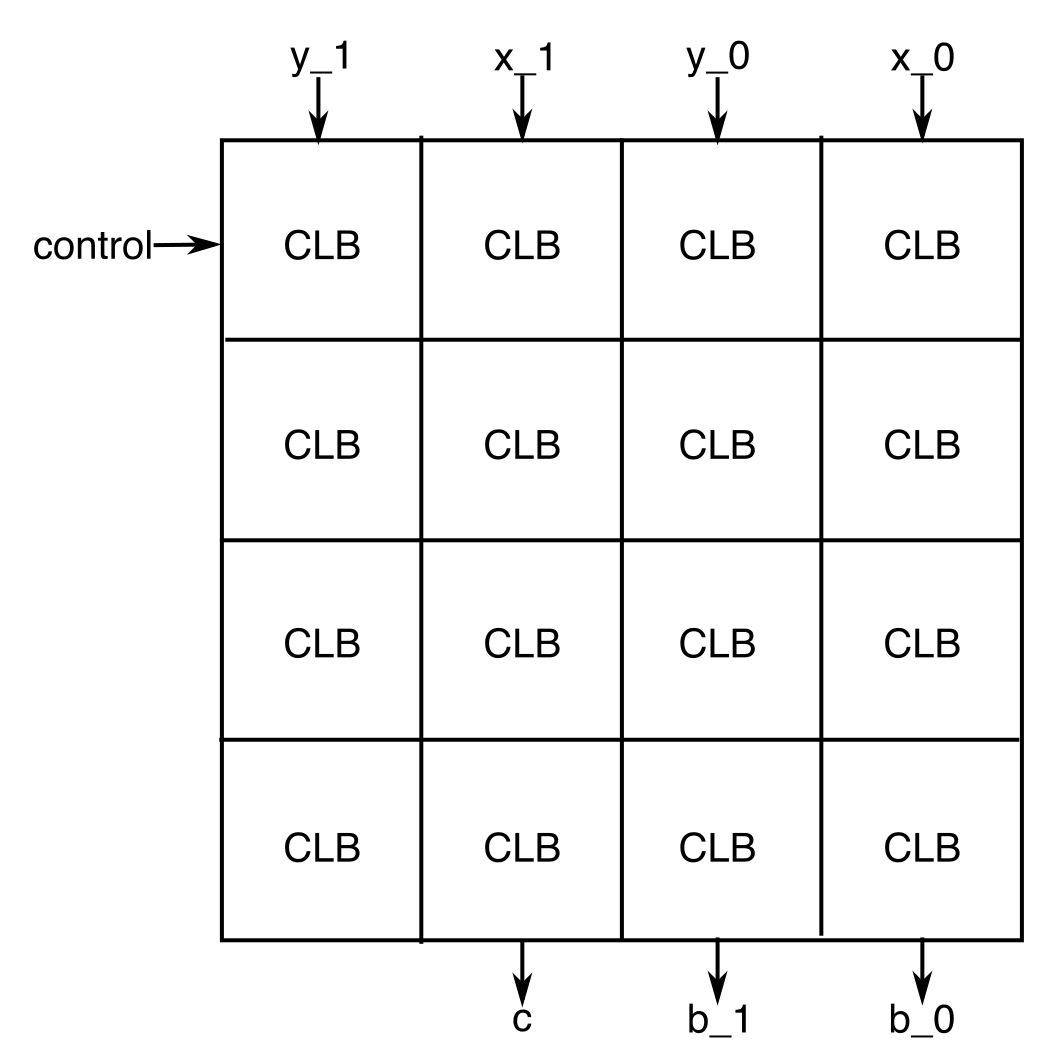
\includegraphics[width=0.6\textwidth]{evaluation.png}
\caption{Diagram detailing how evaluation parameters are fed into the FPGA and answers
read off for a 2-bit arithmetic problem}
\label{fig:control}
\end{figure}

Figure~\ref{fig:control} demonstrates the framework evaluating a 4x4 FPGA attempting
binary arithmatic. Two 2-bit numbers, $x$ and $y$ are deconstructed into their constituent
binary values $\{x\_0,x\_1\}$ and $\{x\_0,x\_1\}$ where $x = x\_0 + 2^{x\_1}$ and $y = y\_0 + 2^{y\_1}$,
these are made available
to the top row of FPGA cells from most significant to least significant bit, and a
control bit (indicating addition or subtraction) is presented to the top left cell.
After FPGA evaluation has concluded 3 bits are read from the bottom, the two bits
constituting the 2-bit answer ($b_0$,$b_1$) and the carry out bit.

The FPGA initialisation step is essential to ensure a deterministic evaluation
process. Without the initialisation, depending on the order in which evaluations
are performed the FPGA can settle on an correct (or incorrect) output dude to the
time taken for new values to propegate through the circuit. This leads to identical
configurations which receive wildly different scores in two evaluations.

\subsection{Fitness Landscape}

When tackling a genetic problem it is important to have an underlying appreciation
for the space of potential answers and how these are related to one another.
In the case of evolutionary hardware
mapping the entire search space is unfeasible, even for a relatively small
FPGA configuration.
The genetic material describing a 4x4 FPGA
is 32 bytes long, therefore there are $2^{32\cdot8}$ potential solutions, any
enumerated bruteforce search processes can only uncover a
miniscule, uninteresting and unrepresentative corner of the fitness landscape
within any reasonable timeframe.

Furthermore each CLB has 7 axes of freedom, multiplying this across the entire 4x4 FPGA
there are 112 dimensions. Visualsing a fitness landscape which exists in
112 dimensions is near impossible. In order to gain a better understanding
of the nature of the underlying landscape a measure of the systems ``ruggedness"
is taken, as defined by Barnett \cite{barnett2008ruggedness}. For mutation rate
$M$, fitness function $f()$, mean mutant fitness function $\mu()$, covariance and
variance functions $cov()$ and $var()$, Equation~\ref{equ:rugged} details how to
calculate ruggedness at a specific mutation rate, $\rho(M)$.

\begin{equation}
	\rho(M) = \frac{cov(f(g),\mu(g)))}{var(f(g))}
	\label{equ:rugged}
\end{equation}

This exercise highlights the nature of the underlying landscape and the function
traversing it.
This ruggedness measure is equivalent to the correlation between an individuals
fitness and the fitness of any offspring it produces\footnote{The genetic algorithm
used to gather the data was calibrated with; a population
size of 50, elitism, tournament selection of size 20, probability of crossover 0,
a multiobjective-fitness function incoperating diversity weighted at 20\% accuracy,
(see Section \todo ref), and the mutation rate varied between experiments. This parameter
configuration was arrived at after the experimentation in Chapter~\ref{chap:evaluation}.}.
Figure~\ref{fig:rugged} outlines the relationship between the mutation rate and
ruggedness. Even with a small number of mutations the correlation between parents
and their children is ambysmally small. As the mutation rate aproaches 3 this correlation
reaches a value of 0.1. This highlights the expected failure rate in an individuals children
and the infrequency of viable individuals.


\begin{figure}
	\centering
	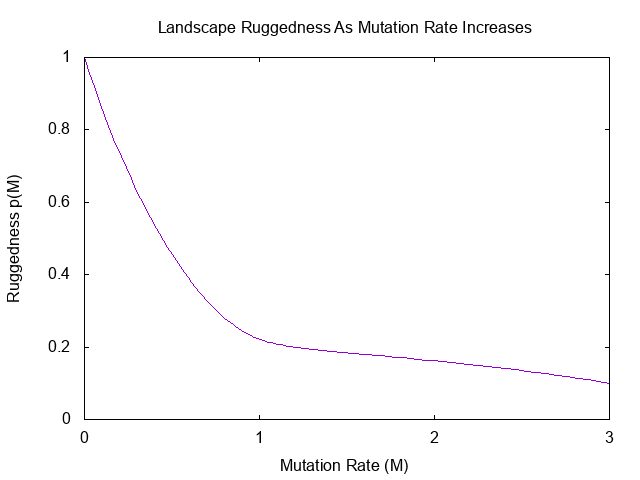
\includegraphics[width=0.5\textwidth]{rugged.png}
	\caption{Landscape ruggedness at different mutation rates}
	\label{fig:rugged}
\end{figure}

\todo fix this next paragraph

In keeping with problems often tackled by genetic algorithms the landscape implied by Figure~\ref{fig:rugged}
is discontinuous
and random. Despite this however,
the landscape is one which doesn't necessarily lend itself to easy searching via genetic algorithm.
It is covered in local optima and the peaks are sharp, unpredictable, and not uniformly
distributed. Therefore solutions will often be local optima, and successful solutions will
be fragile, not taking much mutating to be cast back into the primordial soup.

An ideal fitness landscape for genetic algorithms is one which has gentle hills
which can be ascended, where aggressive mutation does little to render a potential
solution inert. However, the landscape hinted at in Figure~\ref{fig:rugged} is
one which there are few effective mechanisms to navigate, the current ideal resting
with a highly targeted genetic algorithm.

\subsection{Genetic Algorithm}

The basis for the genetic algorithm follows similar work done by Adrian Thompson
\cite{10.1007/3-540-63173-9_61}, but with a number of alternate avenues explored
for problem specific improvements.

\paragraph{Parameter choices}
The basic genetic algorithm has a number of interplaying parameters which affect the genetic
process in some interesting ways. Population size is one such parameter which we must consider,
the number of individuals in each generation can drastically effect execution. As you grow the
population you improve the probability of finding a solution by a given generation, but this has
diminishing returns and makes the evaluation time considerably more laborious. A smaller population
tends to be less diverse and is more easily dominated by a single effective solution
and it's descendants.

Another important variable in the genetic process is the mutation rate, this defines the
frequency with which we are to expect mutations in the offspring of a given generation.
With a high mutation rate one climbs the evolutionary ladder quicker and can make larger
leaps across a chasm of low fitness. However in less robust populations a high mutation rate
can eradicate fragile solutions leading to a weak population never capable of
climbing to the narrow peak of high fitness.

\paragraph{Selection mechanism}
\todo why do we ignore stochastic selecton
The primary selection method will be rank-based selection, which is by far
the most popular selection method observed in preexisting work, however,
tournament selection will also be explored.

Rank-based selection is performed primarily by ordering the members of a population
based on their fitness and then associating the probability of selection to a
linear function on the
position within the ranking. By adding a "skew" by shifting the probability function
to one closer resembling a quadratic one can emphasise the best performing
individuals over the more balanced linear selection function.

A single parameter change allows us to change the relative weightings of high scoring
and low scoring individuals in a population via Equation~\ref{equ:skew}. Given
population size $n$, individual $x$, the individuals position in the ranking $r$, and
skew $s$ (between 0 and 1, where 1 is linear selection and 0 is quadratic) it
generates a score between 1 and the population size plus 1. By varying the skew
value I hope to gain insight into the impact of a more or less discriminatory
selection mechanism.

\begin{equation}
	\label{equ:skew}
	P(x) = \frac{2}{n(n+1)} (\frac{1-s}{n}r^2 + sr + 1)
\end{equation}

Tournament selection involves randomly selecting $k$ individuals from the
population, and the one with the highest fitness is chosen to fill a place
in the new generation. The process is repeated until the new generation is
sufficiently populated. This adds another element of randomness to the
genetic process, giving poorer solutions an opportunity to be in a tournament
with other poor solutions and therefore has the ability to improve the
diversity of the new population at the expense of running the risk that
better solutions might be chosen for tournaments infrequently (or not at
all).

Roulette wheel selection is not well suited for the task of binary addition
within evolvable hardware. The fitness increases associated with a slight
improvement in the design are huge, and this often leads to marginally better
solutions eclipsing solutions which given more time could have evolved into
equivalent (or even improved) solutions.

\paragraph{Elitism}

Selection will also incorporate elitism, this directly copies the best individual
to the next population and ensures that the most fit member
of the population is preserved unmolested by mutation. The fragility of potential
solutions has been highlighted by Figure~\ref{fig:rugged} and highlights the
need to employ some preservation mechanisms.

\paragraph{Multi-objective Fitness Function}
\todo Reference forwards, early testing demonstrated the need for a diversity
measurement, see page ...

Extending the generic fitness function to a linear combination of multiple different
functions applies evolutionary pressure to a multitude of useful different factors.
For evolvable hardware the most important are often correctness and size.

A small design is desirable as the smaller a design is the less power consumed
by the device. To encourage smaller configurations a fitness functions can
incorporate the number of cells inactive in a design into the evaluation
procedure.

Given the large volume of local optima and irregular peaks in the fitness
landscape as demonstrated by Figure~\ref{fig:rugged}, it may be prudent to
also incorporate some measure of diversity. \cite{deJong:2001:RBP:2955239.2955241}
proposes a using a
distance measure from each individual to each other individual in the population
to generate a score for the mean squared distance from a given member of the
population to the rest of the population. This metric can be incorporated into
the multi-objective fitness function to preserve designs based on novelty alone.
These novel designs continue to experience evolutionary pressure and a series
of distinct optima should exist within the population, improving the probability
that the system avoids evolutionary deadends and discovers a working solution.

The proposed diversity metric does not scale well as the population size increases
as with a population size of $n$ the evaluation step requires $O(n^2)$ individual
distance measurements.

\begin{equation}
	\label{equ:multi}
	f(x) = w_{correct} \cdot f_{correct}(x) + w_{size} \cdot f_{size}(x) +
	w_{div} \cdot f_{div}(x)
\end{equation}

Equation~\ref{equ:multi} summarises the multi-objective fitness function around
which this evolvable hardware system is developed, where $w_x$ is the weighting
associated with the fitness function $f_x$. $f_{correct}$ is the original fitness
function of the process, $f_{size}$ is a measure of how small and efficient a
solution is, and $f_{div}$ provides the mean distance from an individual to
every other individual in the population. If a population has a high $f_{div}$,
the population is diverse.
The weightings are all
configurable and allows for fine grain sculpting of the evolutionary process.
The size metric ensures power efficient solutions, and the diversity encourages
a genetic variety. These need to be balanced with the weight given to solutions
to be correct, it should be more important to be correct than small, for example.

\paragraph{Crossover}
Early experiments will be conducted without any crossover mechanism, and therefore
asexual reproduction (individuals will only have a single parents). But single
point crossover will eventually be included and a range of crossover probabilities
will be investigated.

After selection the new population of strings will be randomly paired up, and given
a probability will undergo single point crossover. If crossover is to happen a
random point in the 32 byte string is chosen and the two paired individuals will
swap all values beyond the randomly chosen point. Once the entire population has
undergone a similar procedure the population experiences mutation.

\todo mention this is a non-standard approach but functionally identical

\subsection{Coevolution}

Coevolution will be implemented in a manner similar to the scheme outlined in
\cite{6790490}.
This will allow coevolution to act as an effective method of employing selective
evaluation and evolutionary pressure to a host population in the context of
evolvable hardware. The selective evaluation will both act as a way to more effectively
discriminate between FPGA configurations but also to reduce the size of the
set of evaluation problems and improve scalability.

A separate population of identical size to the core population of FPGA configurations
will be generated at random. Individuals in this population will consist of a small set
of bitstrings of length of $2b$ where $b$ is the number of bits required for
each operand used in the addition (or subtraction). The first half of the problems
will pertain to addition, and the second half represent subtraction problems.
When using coevolution the
evaluation step is slightly modified. To evaluate both the host (FPGA
configurations) and parasite (list of problems) populations each host is randomly
paired with a parasite, and the host is evaluated as before save that the equations
fed into the FPGA are only the ones specified by each item in the set contained within
the parasite. The parasite gains a score of $m - f_{add}(x) - f_{sub}(x)$ where
$m$ is the maximum score possible ($bl$, where $b$ is the number of output bits for
each problem and $l$ is the length of the set of problems contained within a
parasite).

\todo include parasite diagram

Then the parasite population undergoes selection and mutation in an identical
fashion to the host population.

\paragraph{Variable virulence}
By varying the parasite virulence I hope to reduce the intense discrimination
which could lead to population disengagement and would be exasperated by the
fitness landscape fragility. To this end the ability to vary the parasite
aggression is a central feature of the evolutionary system.

After the parasite is initially scored this score is then translated through
a predefined function. The score is divided by the maximum parasite fitness so
the all fitness exists between 0 and 1. Then given a virulence
between 0.5 and 1.0 (where 1.0 is maximally virulent), the score is translated
via Equation~\ref{equ:vir}, where $m$ is the new modified score, $s$ is the
previous score (normalised to be between 0 and 1), and $v$ is the virulence.
This equation is taken from the coevolutionary work done in \cite{6790490}.

\begin{equation}
	\label{equ:vir}
	m = \frac{2s}{v} - \frac{s^2}{v^2}
\end{equation}

\paragraph{Improved scaling}
Coevolution has the potential to improve how an evolutionary hardware system scales.
The literature has extensively explored how to tackle the ballooning search space size
as you increase the scope of the problem being addressed, but little has been done
to improve the scaling of the evaluation function itself. As you increase the scale
of an evolvable hardware problem, the set of test cases grows at an exponential rate.
I suggest that by coevolving a population of problems against a population of FPGA
configurations we can aggressively reduce the number of test cases used for a fitness
evaluation, and therefore improve system scaling.

\subsection{Fault Modelling}
In order to explore the capacity of evolutionary algorithms to design fault
tolerant circuitry and also the use of evolutionary hardware as a fault
recovery mechanism in itself the definition of what constitutes a fault in
this context must be narrowed down. I primerily want to explore faults
generated on a device as it is used, these faults are mainly caused by
component wear out and unpredictable environmental effects, to
this end I will extend the FPGA simulation to model
faults in the internal logic of an FPGA cell. These faults will manifest as clamping
the output of any logic operation to 0, 1, or 2 (which is the value reserved to represent
an undefined value). The evolutionary algorithm is unaware of the
faults, the only perceptible difference is in the evaluation of a population,
which executes as expected and continues to encourage the population to improve in this
new context.

For most of the testing faults will be randomly generated at runtime; a neccessary
feature due to the unpredictable nature of Darwinean search, but for specific
fault recovery cases expected faults can be specified. An interesting case arises when
a model 2-bit adder is embedded in the population, and then a critical fault is
induced. Observing the sharp recovery of the system indicates the potential of
such a fault recovery mechanism.

Along with observing how evolution can help a system recover from a fault, an
analysis into how a system evolves in the presence of intermittent "sticky"
faults could give insight into the uncomfortable world of irregular fault behaviour.
The evaluation backend of the evolvable hardware platform can activate and
deactivate faults as required. Evolving in the presence of such an evaluation
mechanism should gradually encourage a population which can perform well
irrespective of an active fault or not.

\todo add sticky fault state machine

The reason the faults exist is of no consequence to the evolutionary process,
but grounding this exploration in expected fault models will help to generate
practical recovery methods.

\todo cite

\subsection{Dynamic Weightings}
The second set of dynamic problems being explored involves shifting the relative
weightings applied to ADDs and SUBs in the evaluation step during execution. The
automatic reweighting during execution will allow for the modeling of a system
which has shifting execution priority. In order to maintain a balance between
correctness, size, and diversity in the fitness function the weighting associated
with addition and subtraction are changed together, as one increases the other
decreases. This means that once tuned to effective weightings the exploration of
a dynamically shifting problem is unburdened by the complications of a sensitive
fitness function.

Irrespective of the weightings associated with addition and subtraction the
evaluation step collects complete information about the performance of each.
This is then multiplied by the weightings and divided by the sum of the two
weightings. This produces a value within a constant window. The extended fitness
function which was used is given in Equation~\ref{equ:dynamic}.

\begin{equation}
	\label{equ:dynamic}
	f(x) = \frac{w_{add} f_{add}(x) + w_{sub} f_{sub}(x)}{w_{add} + w_{sub}} + w_{size} f_{size}(x) +
	w_{div} f_{div}(x)
\end{equation}

\section{Implementation}
All the flexibility described in the above design criteria is realised by modifying
the headerfiles of my evolvable hardware sourcecode. The implementation was written
in C to ensure efficient execution and quick development cycles. The software can
be cleanly separated into the GUI, the evolution front end, and the FPGA
simulation backend. Collectively they consist of more than 1500 lines of code, with
an extortionate amount of flexibility, capable to scale the size of the FPGA and the
problem well beyond reasonable limits.

\subsection{FPGA Simulation}
The header file for the simulation backend is contained in Appendix~\ref{appx:sim} and shows the
key datastructures and functions exposed to the components performing evolution.
The simulator can convert bitstrings of appropriate length into an FPGA of a
given size, given an FPGA the simulation can also perform evaluations and
simulate faulty logic within any number of cells.

Converting a bitstring to an FPGA is achieved with the function \texttt{bitstring\_to\_fpga},
which takes a pointer to an \texttt{FPGA} struct and a pointer to a char array as arguments.
The cells of the FPGA are iterated over left to right, top to bottom, to fill a shape defined
by \texttt{FPGA\_WIDTH} and \texttt{FPGA\_HEIGHT} and for each cell the next two
bytes are read from the char array. The meaning of the bytes is parsed out and imbedded
in the FPGA struct via an almost direct mapping (north is encoded as 00 in the bitstring,
and is represented as the value 00 in the \texttt{enum} type \texttt{Direction} whenever
a direction is stored on the FPGA).

When evaluating a given input the two values to be operated upon are stored in
the array \texttt{FPGA.input[ FPGA\_WIDTH ]}, then \texttt{evaluate\_fpga} is called.
Each variable and intermediate value
(any value not defining the operation of the FPGA) is intialised to 2 to represent
an undefined value. The simulation then performs a \texttt{tick} step, which iterates over each
cell pulling data from the neighbouring cells, followed by a \texttt{tock} step, which performs
relevent computation and stores output data in relevent output buffers to be read by
the following \texttt{tick} step. These steps continue in turn
until the output is constant (or an iteration cap is reached in which case it halts).
At this point the function returns and the calling entity can inspect cell data and
score accordingly.

The \texttt{tick} step populates each FPGA cells \texttt{n\_in}, \texttt{e\_in},
\texttt{s\_in}, and \texttt{w\_in}, with the relevent data from each neighboring cell.
For example, when assigning \texttt{n\_in} the southern output (\texttt{s\_out})
of the cell to the north is copied in \todo include diagram of this happening.
This occurs for all cells save ones on the edge, if trying
to access a cell beyond the scope of the simulation the variable is assigned the value
representing undefined, 2. This happens uniformly except in the case of the north most cells,
in which cases their \texttt{n\_in} is the relevant value from the \texttt{FPGA.input}
array. Another exception comes of the form of a control signal input; the cell at the top
left is fed a control signal by way of it's \texttt{w\_in} variable, instead of being undefined
it copies the binary value from \texttt{FPGA.control}. This is intended to distinguish
an addition from a subtraction, for an addition the value will be set to either 0 or 1,
and for a subtraction the value will be set to the other, the association has to be
learned by the FPGA configuration during evolution. The way data is made available to an FPGA
is captured by Figure~\ref{fig:control}

\texttt{tock} consults the variables storing information about the operation
performed by the cell, and performs said operation with the relevant $x$\texttt{\_in} variables,
where $x$ represents one of the cardinal direction.
Then each cell's \texttt{n\_out}, \texttt{e\_out}, \texttt{s\_out}, and \texttt{e\_out}
is assigned in accordance with the cells internal mapping (eg. \texttt{n\_out}, the
buffer the cell to the north coppies for it's \texttt{s\_in} value, could be directly
coppied from the function output, or any of the $x$\texttt{\_in} variables).

\todo include diagram for this step too

Deploying this simulation gave subsecond evaluation times for an entire generation of
4x4 FPGAs. These performance benefits, whilst alienating us from the exploitation
of strange undefined behaviour as experienced by Adrian Thompson\cite{10.1007/3-540-63173-9_61}
it did allow considerably quicker software development and the creation of
evolutionary hardware within the strict confines of defined behaviour which
improved the ability to understand the machinations of their success.

\todo a bunch of relevent datastructure diagrams

\subsection{Evolution}
Beyond calls into the simulation backend and inspecting cells after the FPGA
has been evaluated, the evolutionary front end is a distinct entity which operates
almost solely on the abstract bitstrings which constitute the population(s)
being evolved.

\todo talk about datastructures involved, individual, parasite etc. ind has space
for the FPGA struct in it so it doesnt have to be reinstantiated throughout the
process

Initially a population of \texttt{POP\_SIZE} bitstrings of length \texttt{STRING\_LENGTH\_BYTES}
are randomly generated using the pseudorandom \texttt{rand()} syscall, which
(although cryptographically insecure) is suitably random for seeding a random
population. \texttt{STRING\_LENGTH\_BYTES} is defined as \texttt{2 * FPGA\_HEIGHT * FPGA\_WIDTH}.
If \texttt{COEVOLUTION} is defined as \texttt{1} then a population of
parasites of size \texttt{POP\_SIZE}, is also randomly generated. Each parasite
contains an array of size \texttt{PARASITE\_SIZE} containing \texttt{char}s, each of which represents a
challenge posed by the parasite.

The \texttt{evolve} function is passed the randomly seeded population(s) and
curates the evolutionary process. First it randomly seeds an array of potential
faults, these are stored in an array of \texttt{struct}s labeled \texttt{Fault}.
\texttt{Fault} specifies the coordinates of the cell experiencing the fault,
and some auxiliary information depending on the type of fault being simulated.
Whenever an FPGA configuration is created the fault information is coppied into it.
The function then begins on an unending \texttt{while(true)} loop which conducts
the evolutionary process until halted by the user. If coevolving the parasite
population is shuffled and then the each member of the host population is sent
with it's random parasite counterpart to the \texttt{evaluate} step. This function
also requires a pointer to the entire host population. If coevolution is not
happening the function takes a pointer to a dummy parasite instead. When this
function returns the array \texttt{Individual.eval} has been filled. \texttt{eval[0]}
contains the measure of the individuals correctness (already modified by the
weightings given to addition and subtraction), \texttt{eval[1]} denotes the number
of cells on the configuration in the \texttt{OFF} position, and \texttt{eval[2]}
is set to the diversity measurement. While each \texttt{Individual} is
evaluated the mean value for each fitness measurement is collected and the current
most fit individual is kept track of. If coevolving the most fit individual is then
exhaustively tested against all possible input data and the evaluation metrics
are sent to the GUI handler to redraw
the screen. Information about the population fitness, and best case fitness are
logged in an external file. An iteration counter is incremented, the new population(s)
are generated via the \texttt{new\_pop} function and if \texttt{ELITISM}
is defined as \texttt{1} the individual deemed most fit is then coppied directly over
the the 0th element in the new population array.
Then the user input buffer is checked for keyboard input and any relevent
modification made;
'f' activates/deactivates faults, 'd' loads in a perfect adder and assigns highly targeted faults
to act as the fault recovery demonstration, 'r' reseeds the population(s), the
left arrow key shifts the add/sub weightings towards subtraction, and the right
arrow key shifts it towards addition.

\texttt{evaluate} when passed an \texttt{Individual}, a (if not coevolving, dummy) \texttt{Parasite}
and a pointer to the host population populates the evaluation variables in both
the \texttt{Individual} and the \texttt{Parasite}. If not coevolving this is achieved
by first generating the relevent FPGA via the \texttt{bitstring\_to\_fpga} function
and then iterating over all possible inputs, calling \texttt{evaluate\_fpga} and
then reading the required bits from the bottom of the FPGA, one point is given
for each correct bit. This process is completed for both addition and subtraction
and then the weighted average of both is stored in \texttt{Individual.eval[0]}.
Following the evaluation of correctness each cell is iterated over, for every
cell who's function is denoted as \texttt{OFF}, the individual gets 1 point,
and the total is stored in \texttt{Individual.eval[1]}. \texttt{ind\_distance}
gives a measure of the distance between two FPGA configurations, the distance
from the \texttt{Individual} being evaluated and each other individual in the
population is accumulated and the square root mean squared distance is stored
in \texttt{Individual.eval[2]}, this step is an obvious scaling bottleneck but
provides a diversity measurement which vastly improves the chances of successfully
evolving a solution. If coevolving, the set of test additions is defined by the
first half of the \texttt{Parasite} char array, and the set of test subtractions
is defined by the second half of the array. The fitness of an individual is calculated
as before (as the total number of correct output bits) and the parasite score is
given as the maximum score ($bl$ where $b$ is the number of bits checked for each
test, and $l$ is the length of the char array stored in the parasite) minus
the score given to the host individual.

The function \texttt{ind\_distance}
calculates the hamming weight from one FPGA configuration to another. Two
\texttt{Individual}s are passed in and converted into \texttt{FPGA}s via the \texttt{bitstring\_to\_fpga}
function. Then for every
different function and output routing on the configurations, the individuals are 1 further apart.

\texttt{new\_pop} generates a new population of hosts and, if coevolving, parasites.
When coevolving everything done to the host population is mirrored independently
on the parasite population. If using rank-based selection, the population is ordered
based on it's (weighted) fitness; this ordering is conducted via a
population-specific implementation of quicksort. Each population member is associated
a value between $1$ and $n+1$ by the function \texttt{ind\_prob} based on it's ranking
in the population (low fitness individuals have lower rankings), this is the
probability of each individual being selected for the next generation scaled to make
it an integer. Then for each slot in the new population a
random number is generated by \texttt{rand()} between 0 and the sum of all values
generated by \texttt{ind\_prob}.
Starting from zero and the lowest ranked individual, the value given to each population
member is added to the total. If it exceeds the randomly generated number then that
individual is coppied into the open position in the new population. If it does not exceed
the random number the next individual is checked by adding it's value to the running total,
the process is repeated until the random number is exceeded. When all slots in a new
population have been filled the population(s) are mutated. To this end each member is
itterated over and, given an expected mutation rate defined by \texttt{MUTATION} and
genetic material of length $i$, each bit in each individual is flipped with probability
$\frac{1}{i}\texttt{MUTATION}$.

\texttt{ind\_prob} implements Equation~\ref{equ:skew} to skew the ranking to
be more or less discriminatory to highly performing individuals. The skewing
parameter, given as $s$ in the equation is defined by \texttt{PROB\_SKEW} but
this function simply returns it's argument passed through this quadratic equation as
variable $r$.

\todo include graph of selection pressure for different skew values.

In order to store information about the evolutionary process \texttt{log\_data}
writes information about each generation to a \texttt{log.dat} file, which later
can be processed to develop graphs and better understand the quality of the
evolutionary process. The information harvested can be easily modified and
extended but for the most part it has consisted of the mean correctness value
and the correctness of the best case individual.
We are not overly concerned with the total weighted fitness function as we
are using that as a tool to better optimise for correctness; diversity, for
example, is useful for applying evolutionary pressure to preserving a varied
ecosystem but means little for a correct answer and it's effects should be
visible in measuring the correctness alone.

\todo crossover

\todo tournament selection

\todo fancy diagrams

All the evolutionary parameters can be defined at compile time to drastically
alter the execution of the system, all the modifications can be done within
the headerfile \texttt{evolve.h}.

\todo complete function architecture diagram

\subsection{Fault Implimentation}
Faults were implemented by doing a fault pass after each \texttt{tick tock} cycle in
the function \texttt{evaluate\_fgpa} and
overwriting the relevent output of any faulty cells. Before the \texttt{tick} of the
following cycle the predetermined faulty cells have their designated outputs
clamped to a randomly selected value. The fault information is stored in
two arrays within the \texttt{FPGA} struct, the data pertaining to fault
location and effect is stored in an array of type \texttt{Fault}, this has
\texttt{FAULT\_NUM} entries and fully describes the operation of any fault.
A second array of size \texttt{FAULT\_NUM} consisting of integers contains
binary data about whether or not a fault is active on the current evaluation
and controls the execution of the fault pass.

Three types of fault are explored; stuck at 0, stuck at 1, and undefined. In
the first two the result of any logic operation is stuck at a certain value, this
is typical of some sort of short or wearout within a chip. The last type of fault,
undefined faults, always produce a value of 2 (representing undefined) from the function. This means any
output is indiscernible, a value of 2 is always produced by a function if either
of it's inputs are 2s, this models the propagation of uncertainty and a 2 is always
incorrect if read as the answer to a problem from the bottom of the FPGA.

All faults are randomly generated by the \texttt{evolve} function and can be
programmatically activated or deactivated. If the value of \texttt{STICKY} is
set to 1 faults automatically activate/deactivate every 500 generations which
allows for an in depth exploration of the dynamics of evolvable hardware as a
mitigation technique for faults which are sometimes active or sometimes inactive.
This procedure, if allowed to find an always perfect solution, also breeds a solution
which works irrespective of this specific fault. If the fault being modelled is
typical of this hardware this step can be used to develop highly specific
fault tolerant designs.

\subsection{Dynamic Weightings Implimentation}
Programatically or by user input the relative weightings of addition and subtraction
can be shifted mid-execution.

\todo more here

\subsection{GUI}
The user interface is controlled by the simulation backend, which exposes a
series of simple functions to the evolution front end. These exposed functions
allow the triggering of redrawing and reduces the required volume of information
for easy redrawing of the GUI. \texttt{init\_curses} sets up the environment,
\texttt{redraw} called with correct arguments repaints the user interface, and
\texttt{tidy\_up\_curses} cleanly tidies up the GUI.

\begin{figure}
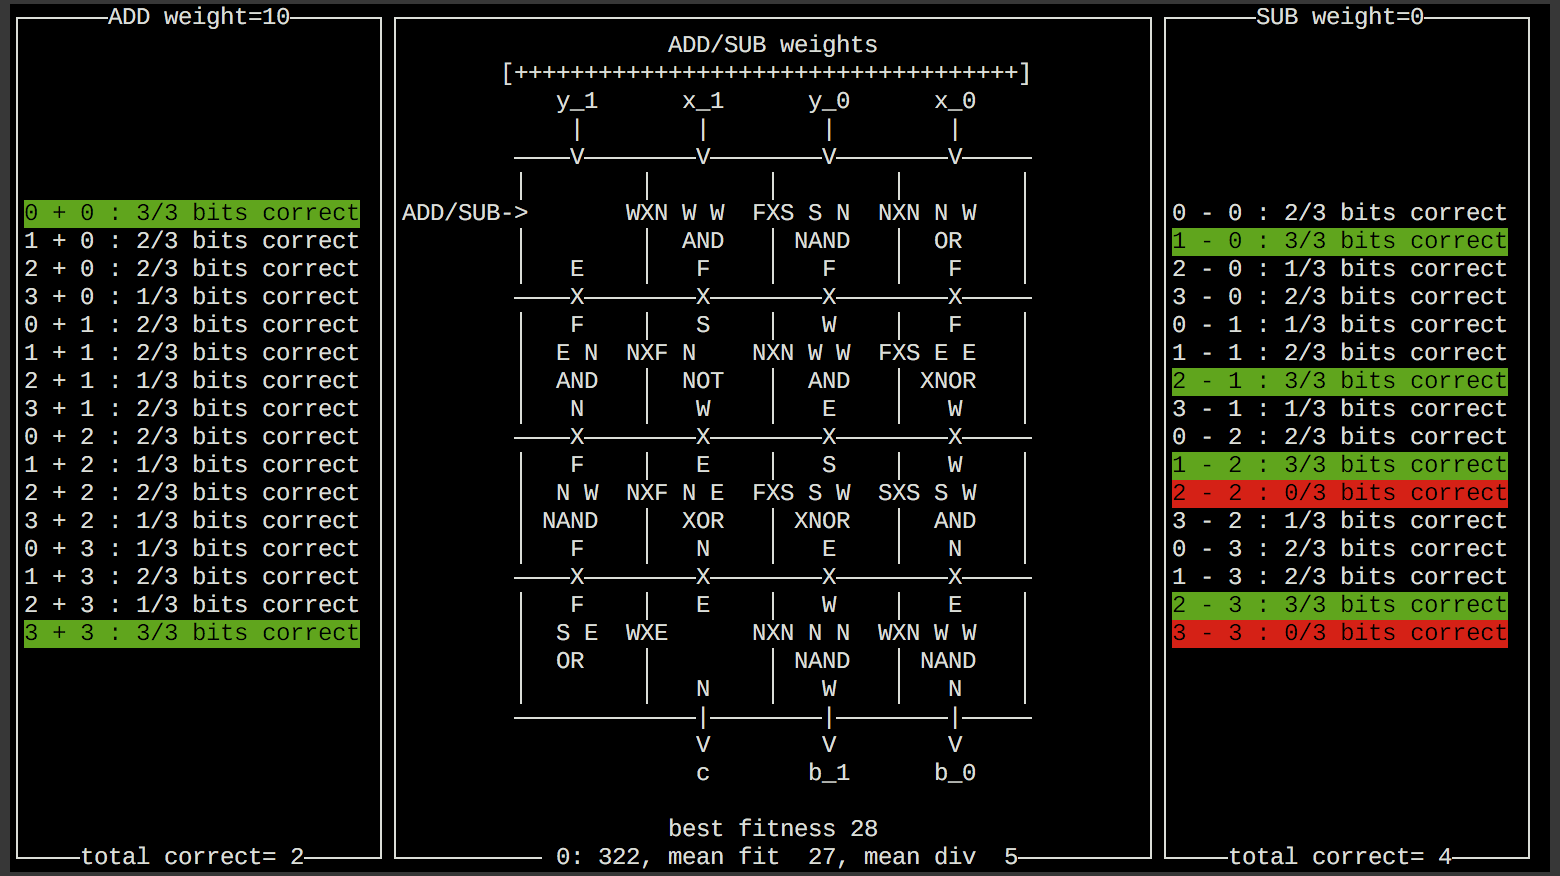
\includegraphics[width=\textwidth]{GUI.png}
\caption{GUI screenshot \todo rescreenshot}
\label{fig:gui}
\end{figure}

The GUI was built with the NCURSES library, a free, open source curses emulation.
It's used to create terminal user interfaces and was chosen due to the amount of
experience  with developing user interfaces with curses, not to
mention a penchant for state-of-the-80s graphics technologies.
Figure~\ref{fig:gui} is a screenshot of the GUI in action. It includes a diagram
of the current best-case FPGA configuration along with it's performance metrics
and information about the underlying population. The panel on the left and right
denote correctly performed addition and subtraction respectively, for a given
if test all 3 bits are correct the test is highlighted in green, if all 3 are wrong
it is highlighted in red.

\todo describe what the gui shows (cell breakdown)

\subsection{Test suite}
The aparatus to perform tests takes the form of a while loop encapsulating the
evolutionary process, reading performance data and meddling with parameters when
required (reseeding the population or changing weightings, for example). The
bounds of the tests being executed are defined in the headerfile \texttt{evolve.h}
(Appendix~\ref{appx:evolve}). \texttt{TEST\_SIZE} defines the number of samples
to be generated, and therefor the number of times the test should be repeated;
\texttt{TEST\_LOOP} defines the size of the inner evolutionary while loop, and
therefore the number of generations each test should be allowed to run for.
During execution information about the best performing individuals, execution time,
and population averages are collected and averaged over each run. This gathered
information is then written to two files \texttt{test.dat}, which involves the
generation-by-generation fitness averages, and \texttt{summary.txt} which details
the number of tests which generated a perfect answer, the average fitness by the
end of execution, and the average execution time.



% -----------------------------------------------------------------------------

\chapter{Critical Evaluation}
\label{chap:evaluation}

{\bf \color{red}A topic-specific chapter, of roughly $15$ pages} 
\vspace{1cm} 

\noindent
{
\color{red}
This chapter is intended to evaluate what you did.  The content is highly
topic-specific, but for many projects will have flavours of the following:

\begin{enumerate}
\item functional  testing, including analysis and explanation of failure
      cases,
\item behavioural testing, often including analysis of any results that
      draw some form of conclusion wrt. the aims and objectives,
      and
\item evaluation of options and decisions within the project, and/or a
      comparison with alternatives.
\end{enumerate}

\noindent
This chapter often acts to differentiate project quality: even if the work
completed is of a high technical quality, critical yet objective evaluation
and comparison of the outcomes is crucial.  In essence, the reader wants to
learn something, so the worst examples amount to simple statements of fact
(e.g., ``graph X shows the result is Y''); the best examples are analytical
and exploratory (e.g., ``graph X shows the result is Y, which means Z; this
contradicts [1], which may be because I use a different assumption'').  As
such, both positive {\em and} negative outcomes are valid {\em if} presented
in a suitable manner.
}

Using the automated testing suite to repeatedly run experiments the data
harvested for the next section
was generated by averaging over 30 independant evolution runs
each for 15000 generations. Each test was aimed at evolving circuitry
capable of 2-bit addition (and later 2-bit addition and subtraction). Evaluation
was performed as outlined in the previous chapter; for each of the 16 tests required
for 2-bit addition the binary representation of each number was made available
to the FPGA and after evaluating the circuitry 3 binary values are read off
the bottom of the grid, for each
correct bit the configuration scored 1 point. For both 2-bit addition and weighted 2-bit
addition and subtraction the maximum score is 48.

Much of the published work in genetic algorithm frames maximising the fitness function
as the aim of genetic algorithm parameter choices. Here most of the data harvested
pertains to the accuracy of the configuration; the number of correct bits read off
the FPGA for each test. This is a measure of how good the configuration is, throughout
execution the fitness function simply acts as an incentive to improve this value.

\todo reference back a lot to other papers

All experiments were conducted on a late 2013 15" Apple MacBook Pro with an
Intel Haswell Core i7 processor clocked at 2.3 GHz and 16GB of RAM.

\section{FPGA Simulator}
The main metric by which to judge the quality of the FPGA simulation is the
speed with which a configuration can be instantiated and evaluated.

\todo actually this

\section{GA Parameter Tuning}
All inital genetic algorithm parameters were set mirroring the parameter choice
of \cite{10.1007/3-540-63173-9_61};
a population size of 50, with elitism, linear rank-based selection, the probability
of single point crossover occuring set to 0.7, and the expected mutations per
offspring set as 2.7. However the problem solved in \cite{10.1007/3-540-63173-9_61}
is dramatically different from the addition problem posed here so a great deal
of domain specific tuning is required. This was chosen as the origin of parameter
exploration as it is paper in the existing literiture which has taken the greatest
pains to explain the experiment configuration and setup.

\todo add more explicit parameters to figure
\begin{figure}
	\centering
	\begin{subfigure}[ht]{0.49\textwidth}
		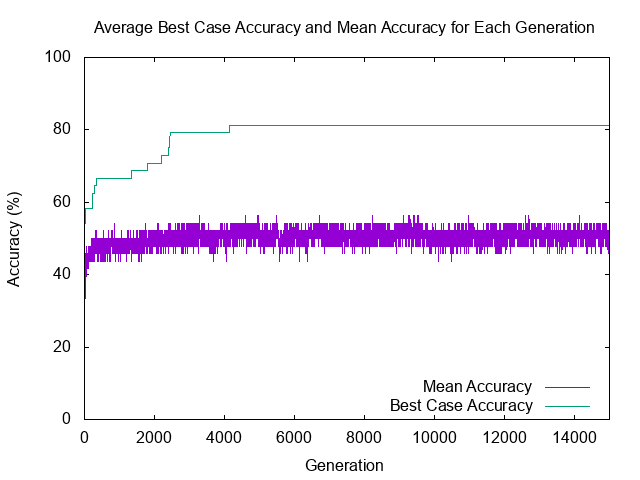
\includegraphics[width=\textwidth]{initial_test.png}
		\caption{}
		\label{fig:initial}
		\vspace{1em}
	\end{subfigure}
	~
	\begin{subfigure}[ht]{0.49\textwidth}
		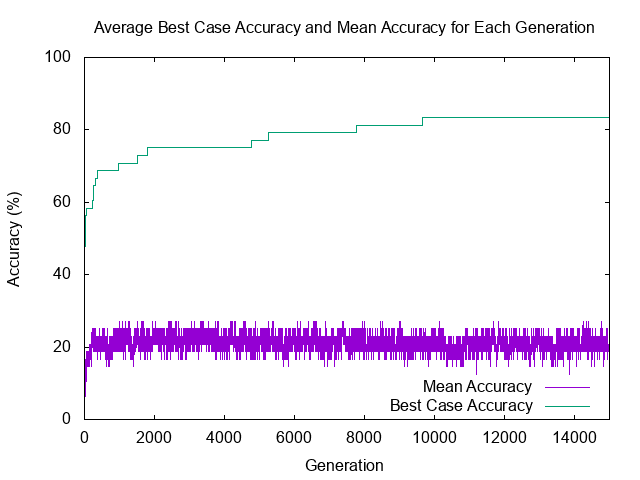
\includegraphics[width=\textwidth]{div_test.png}
		\caption{}
		\label{fig:initial_div}
		\vspace{1em}
	\end{subfigure}
	~
	\begin{subfigure}[ht]{\textwidth}
		\centering
		\begin{tabular}{ccccc}
			\toprule
			& \bfseries{Fitness Function} &
			\bfseries{Perf. Runs (\%)} &
			\bfseries{Avg. Exec. Time (s)} & \bfseries{Avg. Final Accuracy}\\
			\midrule
			(a) & Simple & 0 & 235 & 39\\
			(b) & Multi-Objective & 0 & 267 & 40\\
			\bottomrule
		\end{tabular}
	\end{subfigure}

	\caption[Fitness function test results]{Fitness function test results;
		population size 50, elitism, linear rank-based selection, single point
		crossover probability 0.7, mutation rate 2.7 and
		(a) a simple fitness function mirroring \cite{10.1007/3-540-63173-9_61},
		(b) an extended multi-objective fitness function incorporating a measure
		of diversity with the diversity weight set to 40\% of accuracy.}
\end{figure}

These parameters were evaluated and, as shown in Figure~\ref{fig:initial},
the results of these initial tests are
promising but show a great deal of room for improvement. Despite a healthy
initial improvement in fitness, this quickly reached a plateau and
across the duration of the tests no evolutionary run was
capable of fomulating a perfect solution.
Visual inspection of this initial test as it ran highlighed a huge lack of
diversity in the population of solutions, every improvement in fitness was
an itterative change in the previous best case configuration. This occurs
when a solution improves beyond it's peers and the boost to fertility leads to
it dominating the population. Often a dominating solution will be mostly
correct but due to wildly uneconomic uses of resources be completely incapabale
of evolving any further without dramatic backtracking. The user interface displays
the current average diversity; the distance from one individual to each other in the
population. Relatively early in execution when one member begins to dominate the
diversity plumits.

\todo include proof of plumiting diversity

The diversity in the population averaged (some value), which means that the average number
of different components between an individual and the rest of the population was
as little as 20. With an expected mutation rate of 2.7 this is
indicative of a population completely dominated by a single (potentially bloated)
solution as

\subsection{Improving Diversity}
Such evolutionary
dead ends were also faced by \cite{deJong:2001:RBP:2955239.2955241} who developed
a method of employing multi-objective fitness to encourage population diversity
and minimise waste in solutions. Using their multi-objective fitness function,
a linear combination of diversity and size, to improve the population diversity
and reduce the probability of bloated solutions could provide the evolutionary
pressure required to find a perfect solution. In this situation the final size
of a configuration is inconsiquential, the size is bound to 4x4 and although
a solution which underutilises the FPGA is ideal such stretch goals are beyond
the scope of this document.

A trial was conducted incorporating a diversity measurement weighted at 40\%
of the correctness weighting. This value was arrived at so that diversity,
which exists in the rough range of 0-85, was weighted slightly less than
accuracy, which reaches a maximum of 48.

Figure~\ref{fig:initial_div} dipicts the results from this experiment. Averaged across
repeated executions, there was a slight increase in execution time acompanised by
a marginal improvement in the best case solution fitness
after 15000 generations. However, a larger number of generations was required
to match the accuracy of the simpler fitness function. Despite predictions
to the contrary, another symptom of
the more complex fitness function in this context is a reduced mean population accuracy,
instead of easily beating 20 as happens in Figure~\ref{fig:initial},
\ref{fig:initial_div} maintains a dissapointing
average of 10. This is due to a shift in evolutionary emphasis, in the new
scheme some individuals are given a large fitness due to their novelty alone
and therefore maintained despite their low accuracy, which brings down the
population average. This shift in emphasis also slows the
persuit of perfection; the intial trial in unencumbered with a fitness function
atempting to maintain diversity, and so aggresively persues improvements in
fitness due to a larger proportion of the population which are offspring of a
dominant individual. The slower intial gains in the second trial are indicative
of the smaller segment of the population actively working on the current best
configuration.

These findings disagree somewhat with \cite{deJong:2001:RBP:2955239.2955241},
who found vast improvements across the board when extending the fitness
function. However they did not experiment with population sizes as small
as presented here; unlike our population size of 50, DeJong et al. used
a population size of 1000. It could well be the case that
the population size is too small to facilitate a series of semi-idependently
evolving subpopulations. They also had a mechanism which pruned the population
of ``dominated" individuals which would reduce the tendancy for a population
driven by a fitness function which incorporates diversity to maintain poorly
performing individuals.

To explore this further an experiment with 2 variables was conducted, varying
both the population size (50 and 500) and the incorporation (or not) of a
multi-objective fitness function combining diversity and correctness. A maximum
population size of 500 was used as a
size matching that of DeJong et al. would not feesable in the context as individual
runs would take in excess of 2 hours.

\begin{figure}
	\centering
	\begin{subfigure}[ht]{0.49\textwidth}
		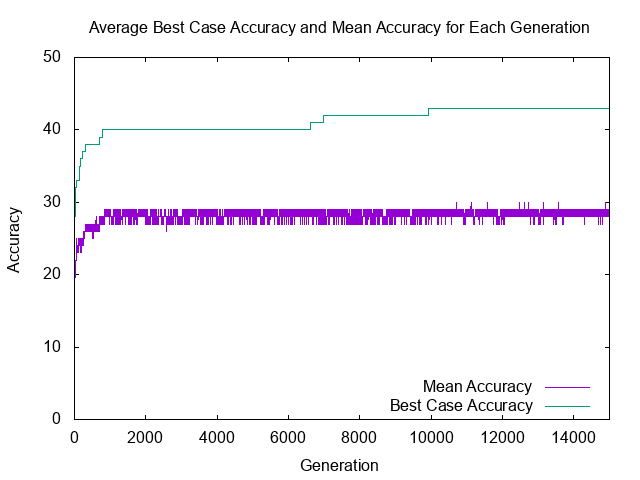
\includegraphics[width=\textwidth]{pop_500_no_div.png}
		\caption{}
		\label{fig:500_no_div}
		\vspace{1em}
	\end{subfigure}
	~
	\begin{subfigure}[ht]{0.49\textwidth}
		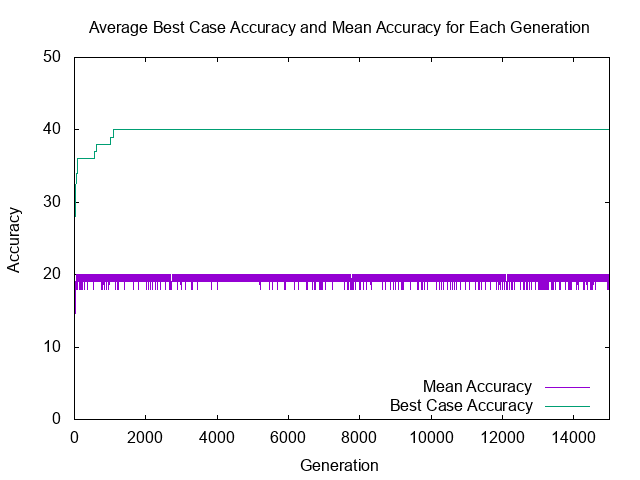
\includegraphics[width=\textwidth]{pop_500_div.png}
		\caption{}
		\label{fig:500_div}
		\vspace{1em}
	\end{subfigure}
	~
	\begin{subfigure}[ht]{\textwidth}
		\centering
		\begin{tabular}{ccccc}
			\toprule
			& \bfseries{Fitness Function} &
			\bfseries{Perf. Runs (\%)} &
			\bfseries{Avg. Exec. Time (s)} & \bfseries{Avg. Final Accuracy}\\
			\midrule
			(a) & Simple & 0 & 2250 & 43\\
			(b) & Multi-Objective & 0 & 2857 & 40\\
			\bottomrule
		\end{tabular}
	\end{subfigure}

	\caption[Large population diversity trail]{Large population diversity trail;
		population size 500, elitism, linear rank-based selection, single point
		crossover probability 0.7, mutation rate 2.7 and
		(a) a simple fitness function mirroring \cite{10.1007/3-540-63173-9_61},
		(b) an extended multi-objective fitness function incorporating a measure
		of diversity with the diversity weight set to 40\% of accuracy.}
	\label{fig:500}
\end{figure}

Figure~\ref{fig:500} contains the results from this experiment. The larger
population size with the simple fitness function (Figure~\ref{fig:500_no_div})
performed the best, the
streamlined persuit of accuracy combined with a larger pool of people to
draw from resulted in the best performance thus far.  The extended function
(Figure~\ref{fig:500_div})
actually reduced the performance, again disagreeing with
\cite{deJong:2001:RBP:2955239.2955241}, and highlighting the
effectiveness of their pruning strategy. This result could be because
the larger population has natural diversity qualities, with a larger pool
a probabilistic procedure such as evolution naturally produces variance,
and the extended
function distracted too much from the persuit of accuracy, and requires a pruning
strategy to reduce waste exploration. The hypothesis
that increasing the population size minimises the reduction in mean accuracy
does ring true. With the smaller population the extended fitness function resulted in
a mean accuracy of less than half the mean accuracy with the simpler fitness function,
whereas
with the a larger population the extended function's trail showed a mean accuracy of
more than
$2/3$rds that of the simpler one.

Despite the improved performance in Figure~\ref{fig:500_no_div} moving forward
further tuning will be performed on the parameters which produced Figure
~\ref{fig:initial_div}. The larger population size in the higher performing experiments
produced an execution time which does not lend itself to exploration and
itterative improvement. Population size will, however, be futher explored in
subsection~\ref{ss:pop_size}.

\subsection{Mutation Rate}

There are two main factors influencing the choice in mutation rate; the fragility
of solutions, and the space between viable individuals. If solutions to a problem are
inherrently fragile, as has been demonstrated in this case by Figure~\ref{fig:landscape},
then a high
mutation rate can regularly destroy working solutions and cause the system to
rarely rise above a fixed value. If the space between viable solutions is vast
a mutation rate which is too small will with low probability cause enough mutations to
span the ravine, yet alone create them in correct places. These two factors are
often at odds, no moreso than in this context, where solutions are brittle and
sparse. Elitism is employed to reduce the impact of fragile solutions by ensuring
the best case solution is never lost, and the inclusion of the extended diversity
fitness function encourages individuals to drift across ravines rather than have
to make the journey in a single step. Therefore the impact of shifting the
fitness function is unclear.

\begin{figure}
	\centering
	\begin{subfigure}[ht]{0.49\textwidth}
		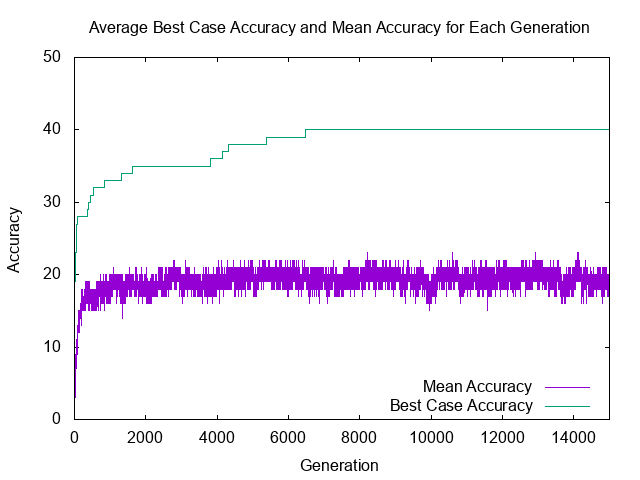
\includegraphics[width=\textwidth]{mut_1.png}
		\caption{}
		\vspace{1em}
	\end{subfigure}
	~
	\begin{subfigure}[ht]{0.49\textwidth}
		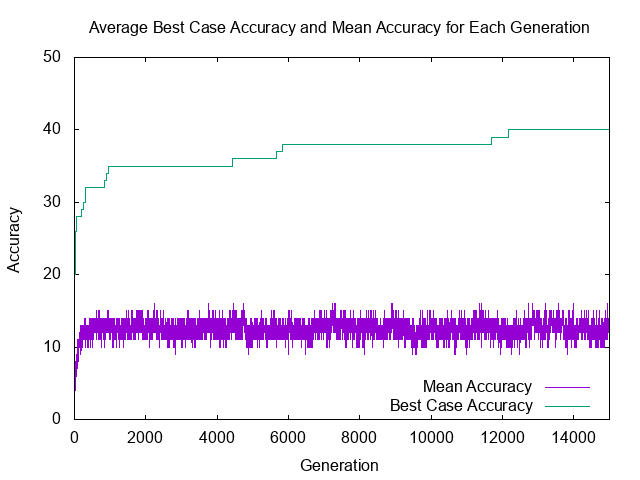
\includegraphics[width=\textwidth]{mut_2.png}
		\caption{}
		\label{fig:mut_2}
		\vspace{1em}
	\end{subfigure}
	~
	\begin{subfigure}[ht]{0.49\textwidth}
		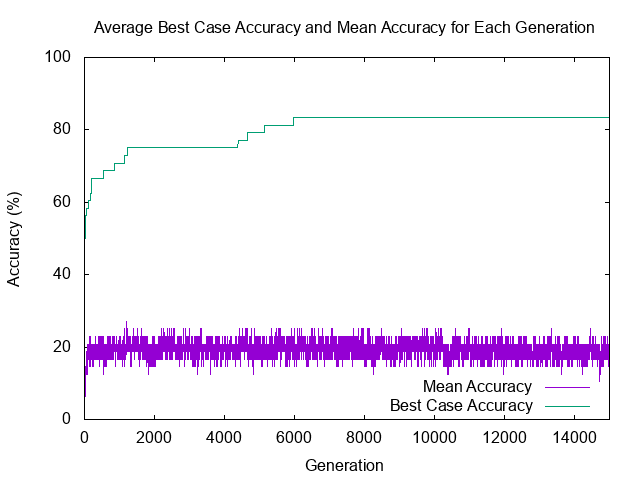
\includegraphics[width=\textwidth]{mut_3.png}
		\caption{}
		\label{fig:mut_3}
		\vspace{1em}
	\end{subfigure}
	~
	\begin{subfigure}[ht]{0.49\textwidth}
		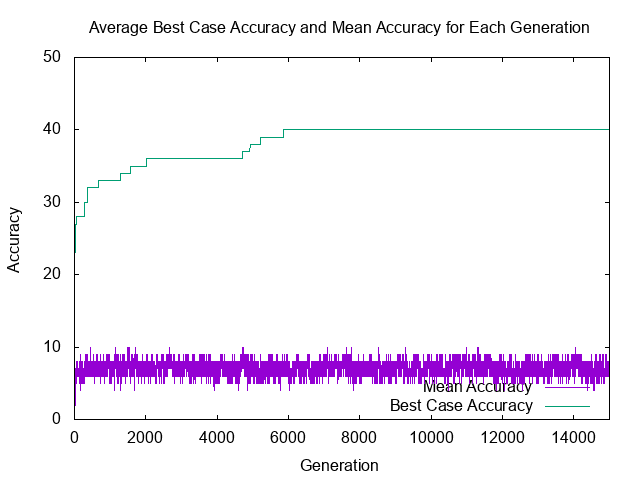
\includegraphics[width=\textwidth]{mut_4.png}
		\caption{}
		\vspace{1em}
	\end{subfigure}
	~
	\begin{subfigure}[ht]{\textwidth}
		\centering
		\begin{tabular}{ccccc}
			\toprule
			& \bfseries{Mutation Rate} &
			\bfseries{Perf. Runs (\%)} &
			\bfseries{Avg. Exec. Time (s)} & \bfseries{Avg. Final Fitness}\\
			\midrule
			(a) & 1 & 0 & 245 & 40 \\
			(b) & 2 & 0 & 264 & 40 \\
			Figure~\ref{fig:initial_div} & 2.7 & 0 & 267 & 40 \\
			(c) & 3 & 0 & 363 & 40 \\
			(d) & 4 & 0 & 368 & 40 \\
			\bottomrule
		\end{tabular}
	\end{subfigure}

	\caption[Mutation rate test results]{Mutation rate test results;
		population size 50, elitism, multi-objective fitness function with diversity
		weighting 40\% of the accuracy, linear
		rank-based selection, single point
		crossover probability 0.7, and
		(a) 1 expected mutation per individual,
		(b) 2 expected mutations per individual,
		(c) 3 expected mutations per individual, and
		(d) 4 expected mutations per individual.}
	\label{fig:mut}
\end{figure}


The experiments conducted in Figure~\ref{fig:mut} mostly agree with the findings
in \cite{10.1007/3-540-63173-9_61} with respect to the experimental results indicating
and ideal mutation rate of around 2.7. However a slight accuracy increase in the
best case individual is
observed when shifting the mutation rate from 2.7 (Figure~\ref{fig:initial_div})
to 3 (Figure~\ref{fig:mut_3}). This is another example of domain specific experimental
tuning for the binary arthmatic problem. The drastic reduction in the speed with which
the best case individual is evolved occuring with a mutation rate of 2
(Figure~\ref{fig:mut_2}) is unexpected. This result could be due to the underlying
topography of the solution landscape; viable solutions are rarely 2 changes apart,
and are more frequently distanced at 1, 3, or 4 changes. This would explain this
marginal reduction in evolutionary swiftness. Note the continuous decrease in population mean accuracy
as the mutation rate is increased, the reasons are twofold; firstly, a higher mutation
rate is more likely to induce a change in an accuracy-critical component of the
solution. Secondly, with an extended fitness function maintaining solutions for
novelty value alone, the more aggresive mutation rate is more likely to cast members of the
population into even further unexplored corners of the fitness landscape giving them
an even higher diversity score (and therefore improving their fitness and their staying power),
these solutions can survive without a high accuracy score.

Because of the results demonstrated by Figure~\ref{fig:mut_3}, namely slighly
improved best-case evolution (at the cost of population accuracy), an expected
mutation rate of 3 has been chosen. This was selected over the mutation rate 1
as the higher population accuracy is a symptom of a more localised less varied
population which is cultivated by a gentler mutation rate.

\subsection{Selection Mechanisms}
The most popular selection methods in evolvable hardware by a considerable margin are
rank selection and tournament selection. Thus far we have been using linear
rank selection (mirroring \cite{10.1007/3-540-63173-9_61}). Here the use
of a variable skewed rank selection is emplyed to place higher evolutionary pressure
on the better performing individuals. The variable controlling the linearity
of the selection function can be set such that the probability of selection
grows quadratically rather than linearly as you move up the rankings. To this
end experiments setting this value to 0 (a quadratic selection function with no linear
component), 0.5, and 1
(completely linear) will highlight any impact this has on the system.

Along with this variation, an experiment comparing current best
selection with tournament selection of varying sizes from 10 (20\% the population
size) upto 40 (80\% the population size). The smaller tournament size
will discriminate less against lower performing individuals, and the
larger the tournament the fewer poorly performing configurations will
be selected for the next generation. This interplay could dramatically
increase performance, exploiting a balance (\todo much like cite cite cite)
to drastically improve performance.

\begin{figure}
	\begin{minipage}{\textwidth}
	\centering
	\begin{subfigure}[ht]{0.32\textwidth}
		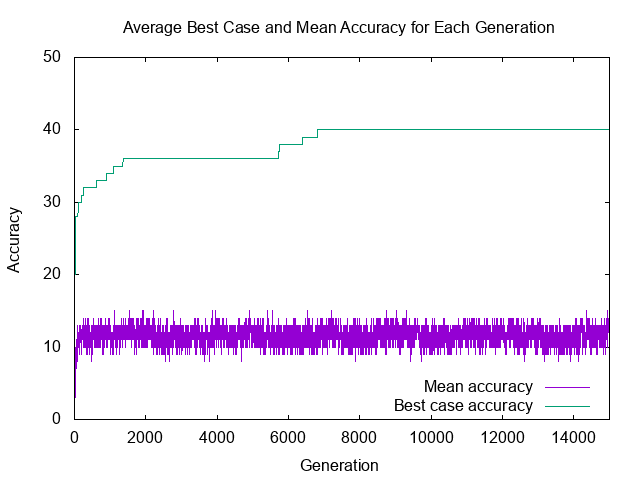
\includegraphics[width=\textwidth]{skew_0.png}
		\caption{}
		\label{fig:skew_0}
		\vspace{1em}
	\end{subfigure}
	~
	\begin{subfigure}[ht]{0.32\textwidth}
		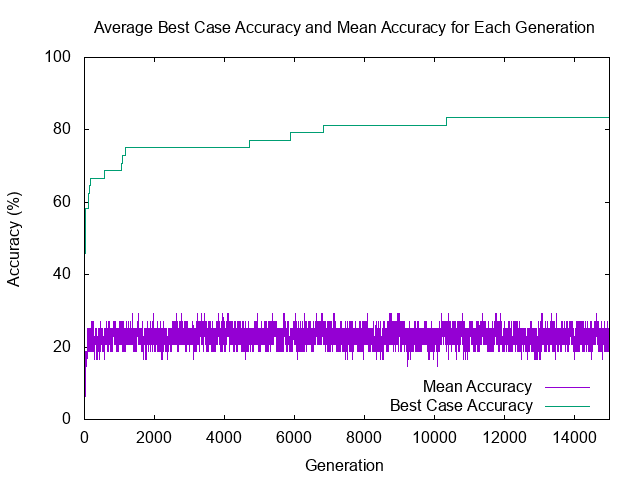
\includegraphics[width=\textwidth]{skew_point5.png}
		\caption{}
		\label{fig:skew_point5}
		\vspace{1em}
	\end{subfigure}
	~
	\begin{subfigure}[ht]{0.32\textwidth}
		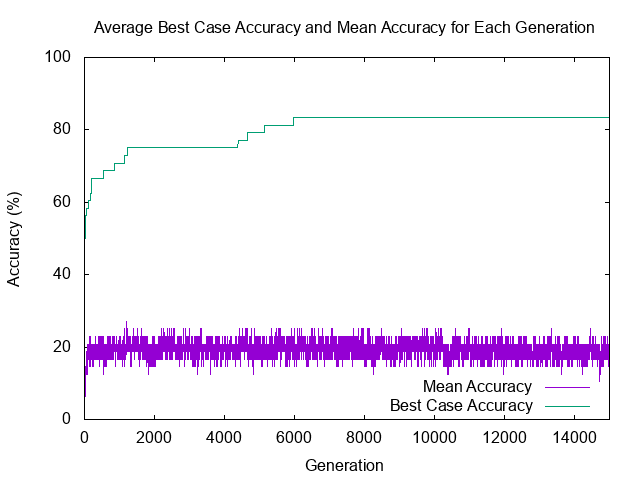
\includegraphics[width=\textwidth]{mut_3.png}
		\caption{}
		\label{fig:skew_1}
		\vspace{1em}
	\end{subfigure}
	~
	\begin{subfigure}[ht]{0.49\textwidth}
		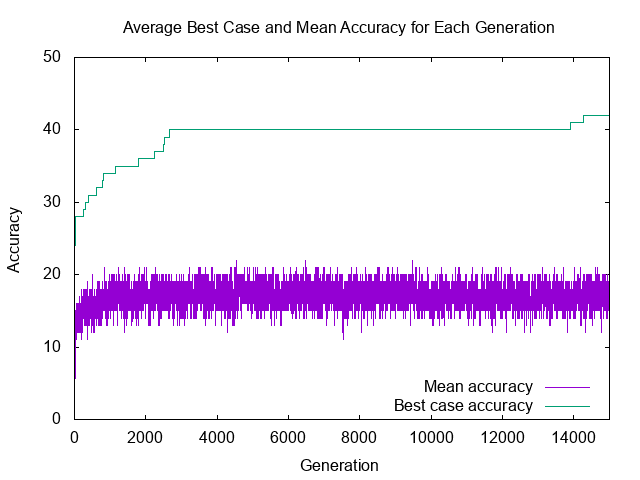
\includegraphics[width=\textwidth]{tour_10.png}
		\caption{}
		\label{fig:tour_10}
		\vspace{1em}
	\end{subfigure}
	~
	\begin{subfigure}[ht]{0.49\textwidth}
		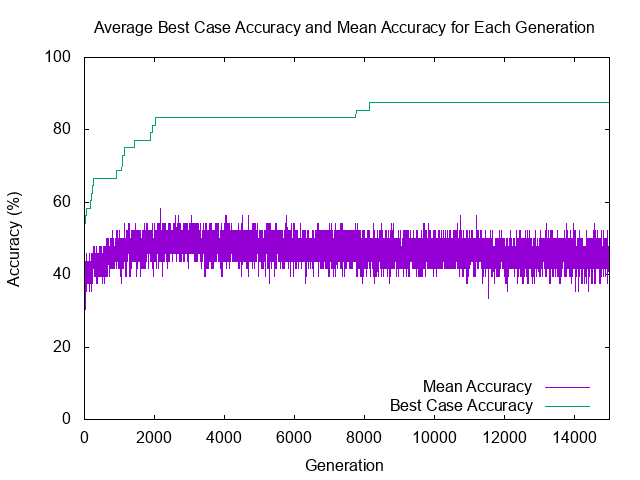
\includegraphics[width=\textwidth]{tour_20.png}
		\caption{}
		\label{fig:tour_20}
		\vspace{1em}
	\end{subfigure}
	~
	\begin{subfigure}[ht]{0.49\textwidth}
		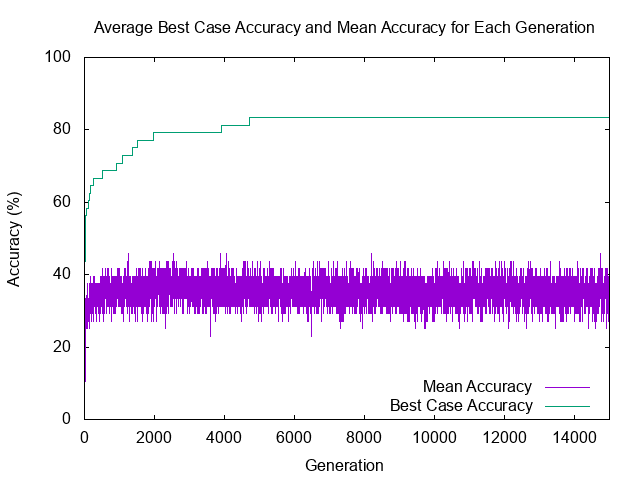
\includegraphics[width=\textwidth]{tour_30.png}
		\caption{}
		\label{fig:tour_30}
		\vspace{1em}
	\end{subfigure}
	~
	\begin{subfigure}[ht]{0.49\textwidth}
		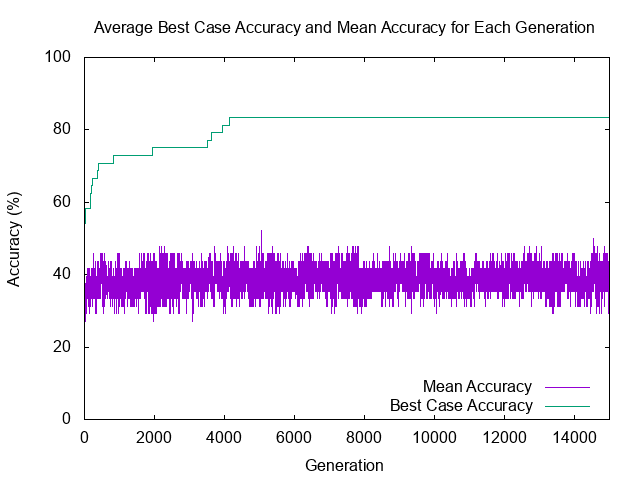
\includegraphics[width=\textwidth]{tour_40.png}
		\caption{}
		\label{fig:tour_40}
		\vspace{1em}
	\end{subfigure}
	~
	\begin{subfigure}[ht]{\textwidth}
		\centering
		\begin{tabular}{ccccc}
			\toprule
			& \bfseries{Selection Method} &
			\bfseries{Perf. Runs (\%)} &
			\bfseries{Avg. Execution Time (s)} & \bfseries{Avg. Final Fitness}\\
			\midrule
			(a) & Rank (Skew 0.0) & 0 & 304 & 40 \\
			(b) & Rank (Skew 0.5) & 0 & 415 & 40 \\
			(c) & Rank (Skew 1.0) & 0 & 363 & 40 \\
			(d) & Tournament (Size 10) & 0 & 264 & 42 \\
			(e) & Tournament (Size 20) & 13 & 231 & 42 \\
			(f) & Tournament (Size 30) & 3 & 260 & 40 \\
			(g) & Tournament (Size 40) & 0 & 244 & 40 \\
			\bottomrule
		\end{tabular}
	\end{subfigure}

	\caption[Selection method test results]{Selection method test results;
		population size 50, elitism, multi-objective fitness function with diversity
		weighting 40\% of the accuracy, single point
		crossover probability 0.7, mutation rate 3 and
		(a)(b)(c)\footnote[1]{(c) duplicated from Figure~\ref{fig:mut_3} for better direct
	visual comparison} rank based
	selection with skew 0.0, 0.5, and 1.0 respectively
	, and (d)(e)(f)(g) using tournament selection with tournament
	size 10, 20, 30, and 40 respectively.}
	\label{fig:select}
\end{minipage}
\end{figure}

The more aggresive discrimination against members of the population due to the
variable skew is clear in Figure~\ref{fig:select}. The population under the more
aggressive selection mechanism (Figure~\ref{fig:skew_0}) persue the
maximum accuracy somewhat quicker than the more linear rank selections
(Figure~\ref{fig:skew_point5} and Figure~\ref{fig:skew_1}), however this
more aggressive discrimination frequently directs the population
with something approaching single-minded determination, often to it's detriment.
The average final fitness is clearly lower with a quadratic rank than with a
linear rank.

Tournament selection with a tournament size of 20 is a clear improvement over
any other selection methods thus far, and has had the single largest impact
on the number of perfect solutions evolved of any parameter choice until
now. 13\% of the trails ended in a perfect solution with an accuracy score of 48.
Individuals are chosen uniformally at random for a tournament, but within a
tournament only the most fit individual wins. This interplay between minimally
and maximally discrimanatory selection schemes results in heavily directed evolutionary
search which maintains a very diverse population. Each of the tournament schemes
have a high population accuracy with a wider variance than any of the rank
selection schemes, indicating the diversity maintainance. The smaller tournament
size, Figure~\ref{fig:tour_10} is too random and does not put enough evolutionary
pressure on finding an accurate solution.
Despite maintaining a broad population the fitness is lower due to this lack of
pressure. The larger tournament size Figure~\ref{fig:tour_40} discriminates too
aggressively, in any selection round the weakest 80\% of the population cannot
be selected (as they are guaranteed to lose the tournament), this leads to a
dominated and ultimately weaker population.
Balancing these two facets of tournament selection, a tournament size
of 20 allows for a search procedure directed enough to find optimal solutions
and with enough random influence to maintain a wide population.

\subsection{Crossover}
Crossover works well in this context, the nature of the mapping between genotype
and phenotype means any crossover can provide benifits to both mating pairs and
inject some much needed diversity into the ecosystem. Three additional trial runs
were execuited, each at a different crossover probability rate; 0, 0.5, and 1.
Crossover points only occur between bytes, never inside them; so
when genetic material is transplanted it is always clean and individual cell
operation is consistent before and after.

\begin{figure}
	\centering
	\begin{subfigure}[ht]{0.49\textwidth}
		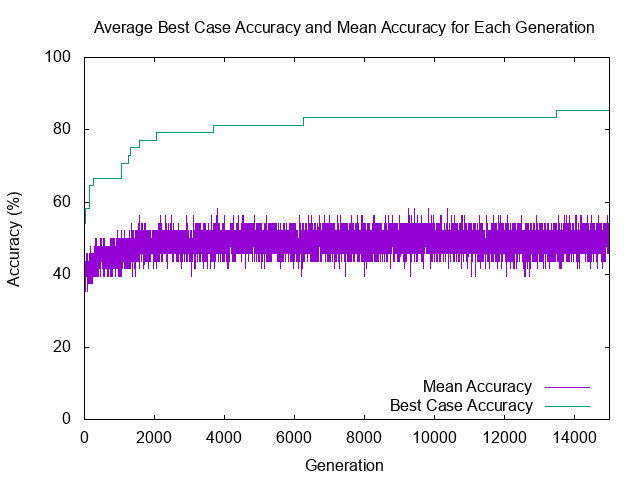
\includegraphics[width=\textwidth]{cross_0.png}
		\caption{}
		\label{fig:cross_0}
		\vspace{1em}
	\end{subfigure}
	~
	\begin{subfigure}[ht]{0.49\textwidth}
		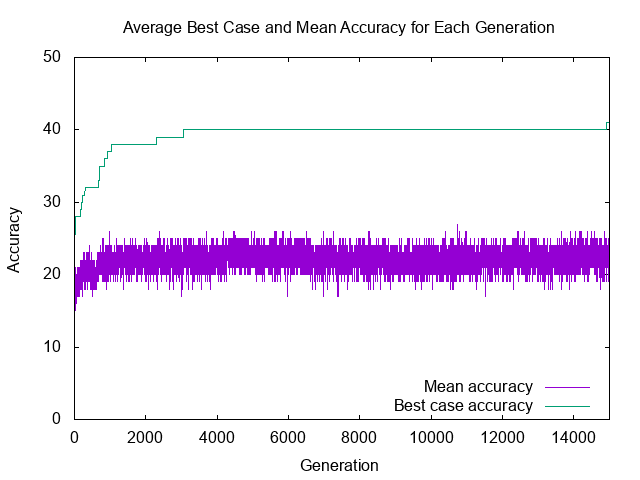
\includegraphics[width=\textwidth]{cross_point5.png}
		\caption{}
		\label{fig:cross_point5}
		\vspace{1em}
	\end{subfigure}
	~
	\begin{subfigure}[ht]{0.49\textwidth}
		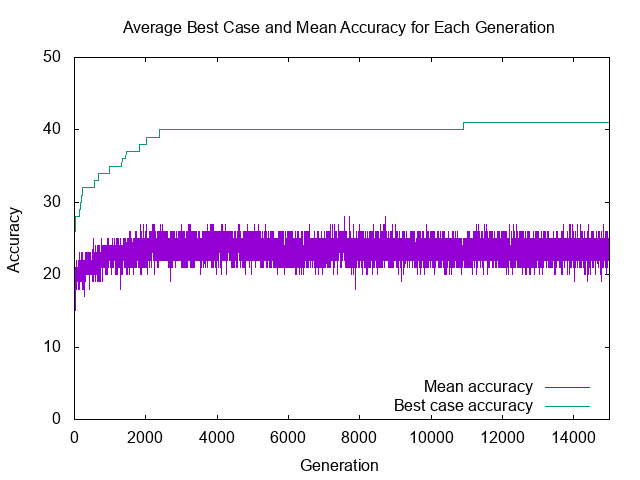
\includegraphics[width=\textwidth]{cross_1.png}
		\caption{}
		\label{fig:cross_1}
		\vspace{1em}
	\end{subfigure}
	~
	\begin{subfigure}[ht]{\textwidth}
		\centering
		\begin{tabular}{ccccc}
			\toprule
			& \bfseries{Crossover Prob.} &
			\bfseries{Perf. Runs (\%)} &
			\bfseries{Avg. Exec. Time (s)} & \bfseries{Avg. Final Fitness}\\
			\midrule
			(a) & 0.0 & 10 & 243 & 41\\
			(b) & 0.5 & 3 & 245 & 41\\
			Figure~\ref{fig:tour_20} & 0.7 & 13 & 231 & 42 \\
			(c) & 1.0 & 3 & 249 & 41\\
			\bottomrule
		\end{tabular}
	\end{subfigure}

	\caption[Crossover probability experiment]{Crossover probability experiment;
		population size 50, elitism, multi-objective fitness function with diversity
		weighting 40\% of the accuracy, mutation rate 3, tournament selection of size
		20, and probability of single point crossover set to (a) 0.0, (b) 0.5, and (c) 1.0.}
	\label{fig:cross}
\end{figure}

In Figure~\ref{fig:cross}, none of the trails produced results rivaling the
initial crossover probability
of 0.7. This behaviour could be a result of how crossover influences the underlying
population structure; never performing crossover and usually performing crossover
performed better than always performing crossover an performing or not with an equal
probability. An explination for the performance at 0 probability could be that
when the population develops without the threat of crossover there is an implicit
encouragement to diversify as there is no punishment for creating a novel solution
which crossover would destroy by mating with an uncompatible partner. Poor performance
at equal probabilities could be a symptom of the same behaviour; when crossover
may or may not happen with equal probabilities a population cannot adapt either way.
The poor performance at 100\% probability would seem to disagree with this, unless you
consider that crossover is ultimately a disruptive force. When crossover is guaranteed
the population can only develop solutions durable in the face of random string swapping.
0.7 provides a good balance where a population can develop with the assumption of
crossover but there is a chance solutions can develop which rely on crossover not
happening.

\subsection{Elitism \label{ss:elitism}}
With a mutation rate as high as shown here the effect of elitism is hightened.
The probability of a mutation crippling a design is relatively high and so a population
without elitism is prone to climbing the evolutionary ladder just to be cast
down by luck. Binary arithmatic is especially fragile, as demonstrated by Figure~\ref{fig:no_elitism},
where the evolutionary parameters are consistent with our highest performer so far, except
elitism is turned off.

\begin{figure}
	\centering
	\begin{subfigure}[ht]{0.49\textwidth}
		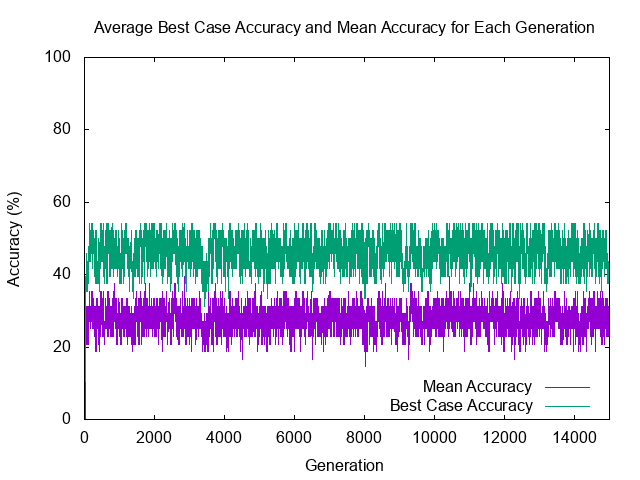
\includegraphics[width=\textwidth]{no_elite.png}
		\vspace{1em}
	\end{subfigure}
	~
	\begin{subfigure}[ht]{\textwidth}
		\centering
		\begin{tabular}{ccc}
			\toprule
			\bfseries{Perfect Solutions (\%)} &
			\bfseries{Avg. Execution Time (s)} & \bfseries{Avg. Final Fitness}\\
			\midrule
			0 & 281 & 19\\
			\bottomrule
		\end{tabular}
	\end{subfigure}

	\caption[Removing elitism test results]{Removing elitism test results;
	population size 50, no elitism, multi-objective fitness function with
	diversity weighting 40\% of the accuracy, mutation rate 3, tournament
	selection of size 20, and probability of single point crossover set to 0.7.}
	\label{fig:no_elitism}
\end{figure}

Clearly, as Figure~\ref{fig:no_elitism} demonstrates removing elitism is crippling.
The population rarely, if ever, performs better than an accuracy of 28. From here
the any path to a better viable solution is insurmountable, crippled by an aggresive
mutation rate, which explored the search space with such vigor that no individuals
performing well can survive due to their inherrent fragility. This dissagrees with
(\todo cite the natural fault tollerence) which claims evolution naturally discoveres
solutions resistant in the face of change; for binary arithmatic the solutions are
too fragile to have such a resistance and require the support of elitism to prop
up the best individuals. Resulting in solutions which do not have the same durability
as a solution found without elitism, if one could ever be found.

\subsection{Tuning Population Size \label{ss:pop_size}}

With the desire to cultivate a diverse population at the forefront of the parameter
selection reasoning enlarging the population would improve the spread of solutions,
and allow the evolutionary pressure on diversity to simultaneously mature and
develop a bredth of solutions.
Obviously increasing the size of the population has objective benifits in a statistical
sense, by casting the net wider there is a higher chance to stumble
accross the correct solution.
But, this has diminishing returns; due to the diversity measurement incorporated into
the fitness function the evalutation time grows with $O(n^2)$ complexity with the
population size.

The increased population size from the experiments with a multi-objective
fitness function could be beyond the point of diminishing returns. To explore this
further trials varying the population size to explore how execution time and
genetic algorithm performance is affected. Population sizes of 25, 50, 100, and 200
were selected to span the bredth of potential choices. For each the tournament size
scaled acordingly, constantly set to 40\% of the whole population (10, 20, 40, and
80 respectively).

\begin{figure}
	\centering
	\begin{subfigure}[ht]{0.49\textwidth}
		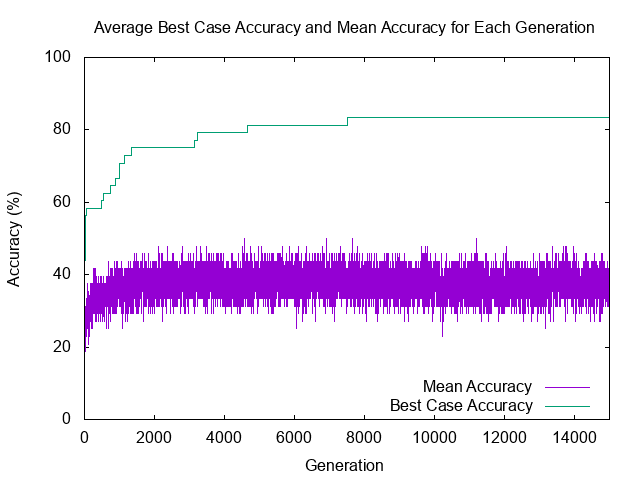
\includegraphics[width=\textwidth]{pop_25.png}
		\caption{}
		\vspace{1em}
	\end{subfigure}
	~
	\begin{subfigure}[ht]{0.49\textwidth}
		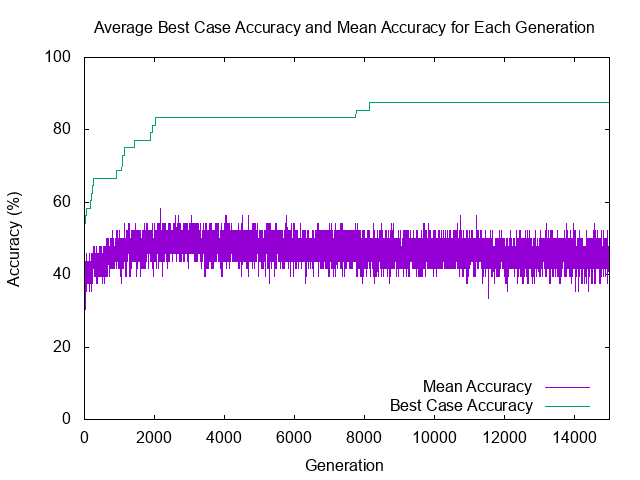
\includegraphics[width=\textwidth]{tour_20.png}
		\caption{}
		\vspace{1em}
	\end{subfigure}
	~
	\begin{subfigure}[ht]{0.49\textwidth}
		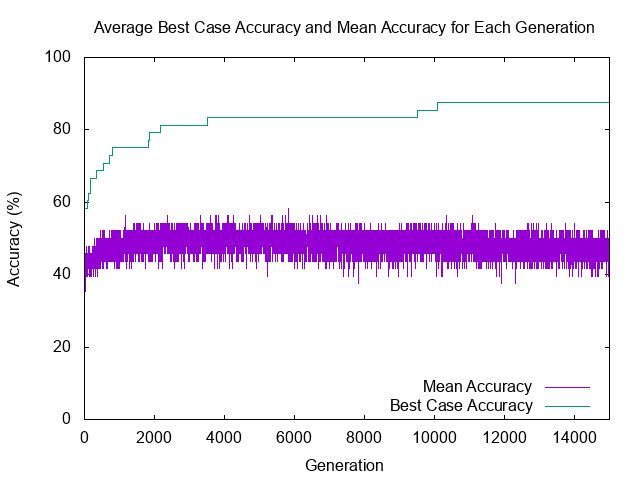
\includegraphics[width=\textwidth]{pop_100.png}
		\caption{}
		\vspace{1em}
	\end{subfigure}
	~
	\begin{subfigure}[ht]{0.49\textwidth}
		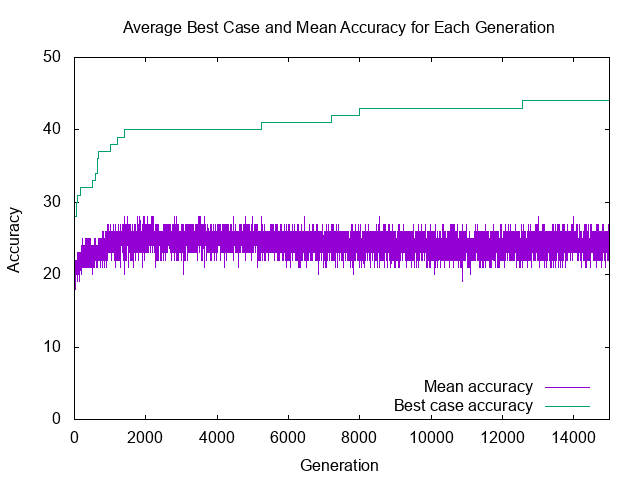
\includegraphics[width=\textwidth]{pop_200.png}
		\caption{}
		\vspace{1em}
	\end{subfigure}
	~
	\begin{subfigure}[ht]{\textwidth}
		\centering
		\begin{tabular}{ccccc}
			\toprule
			& \bfseries{Population Size} &
			\bfseries{Perfect Solutions (\%)} &
			\bfseries{Avg. Execution Time (s)} & \bfseries{Avg. Final Fitness}\\
			\midrule
			(a) & 25 & 0 & 126 & 40\\
			(b) & 50 & 13 & 231 & 42\\
			(c) & 100 & 17 & 457 & 42\\
			(d) & 200 & 57 & 955 & 44\\
			\bottomrule
		\end{tabular}
	\end{subfigure}

	\caption[Population tuning test results]{Population tuning test results;
	elitism, mutli-objective fitness function with diversity weighting 40\%
	of the accuracy, mutation rate 3, tournament selection of size 40\%
	the population size, probability of single point crossover 0.7, and
	(a) population size 25, (b)(duplicated) population size 50, (c) population size 100,
	and (d) population size 200.}
	\label{fig:pop}
\end{figure}

Unsurprisingly the larger population has the highest average final fitness,
and proportion of evolutionary runs ending in a perfect solution but
Figure~\ref{fig:pop} highlights an interesting revelation; Despite the evaluation
function scaling with complexity $O(n^2)$ the increase in execution time is
almost linear with the population. This indicates the poorly scaling portion of
the evalutation function measuring population diversity counts for an insignificant
minority of the execution time. The most aggressive increases in time are due to
the aditional population members which need to be instantiated as FPGAs and
fed the test data. This evidence against the claims made in (\todo ref earlier scaling
claims) demonstrate that the scaling issues are localised to FPGA evaluation.

For all population sizes achieving a best-case accuracy of 36 occured in a
similar amount of time, however the larger populations were able to maintain
this ascent up the evolutionary ladder better. This sudden insummountable
evolutionary barrier for the smaller population sizes implies that the smaller
populations were unable to cultivate a bredth of solutions early in execution
and therefore encountered an evolutionary deadend, temporarily halting improvements.

Moving forward a population size of 50 was selected. Clearly the population size
of 200 is the best candidate, but the increase in persentage of perfect solutions is almost
linear with the added execution time. In order to maintain momentum at this stage
in the project the quicker execution was chosen, with the knowledge that one could
quadrouple the population to increase the execution time and persentage of perfect
solutions by a factor of 4.

\subsection{Tuning Diversity}

One aspect of the evolutionary proccess hitherto unexplored is the relative
weighting given to the diversity measurement in the fitness function. If
set too high the genetic algorithm begins directing for novelty alone,
accuracy is obscured and diversity reigns suprime. If set too low we reenter
the domain of single-minded persuit of accuracy, one which frequently
falls into evolutionary dead ends gracelessly halting progress. Diversity
weighting is defined here as a fraction of the weighting given to accuracy.
Accuracy exists in the range 0-48 for the 2-bit binary arithmatic problem,
and from experimental results diversity usual reaches a maximum value of
around 85. So for any diversity weighting larger than half the size of
the accuracy weighting an individual does well to be maximally diverse,
accuracy occuring as an afterthought. Armed with this knowledge an experiment
was framed running evolutionary
trails at a number of key diversity weightings, 0.0, 0.2, 0.4, and 0.6 accuracy weight.
This shifts evolutionary pressure from completely focussed on accuracy to mostly
completly focussed on diversity.

\begin{figure}
	\centering
	\begin{subfigure}[ht]{0.49\textwidth}
		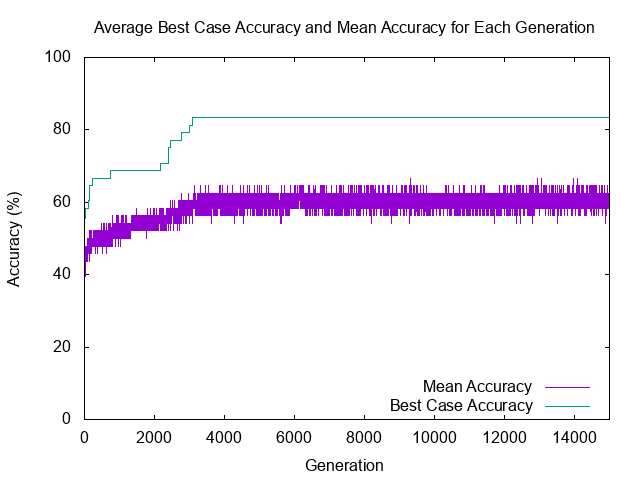
\includegraphics[width=\textwidth]{div_0.png}
		\caption{}
		\label{fig:div_0}
		\vspace{1em}
	\end{subfigure}
	~
	\begin{subfigure}[ht]{0.49\textwidth}
		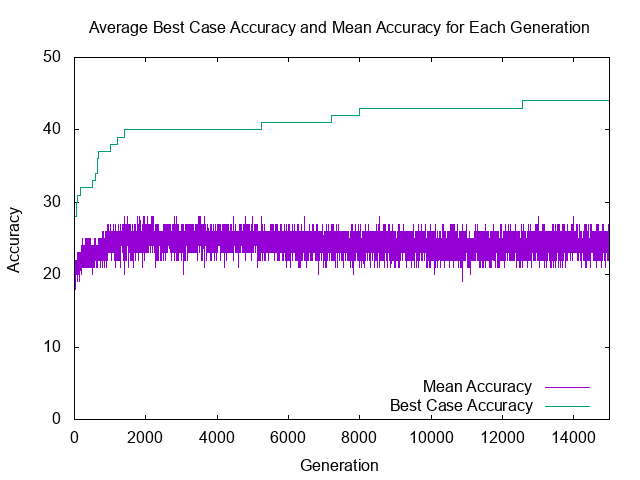
\includegraphics[width=\textwidth]{div_20.png}
		\caption{}
		\vspace{1em}
		\label{fig:div_2}
	\end{subfigure}
	~
	\begin{subfigure}[ht]{0.49\textwidth}
		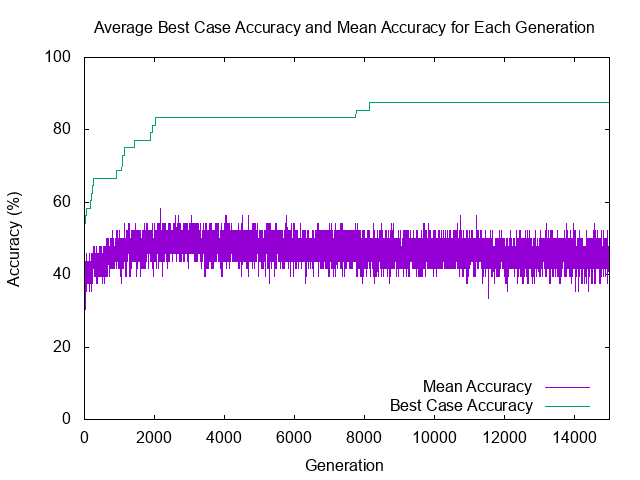
\includegraphics[width=\textwidth]{tour_20.png}
		\caption{}
		\vspace{1em}
	\end{subfigure}
	~
	\begin{subfigure}[ht]{0.49\textwidth}
		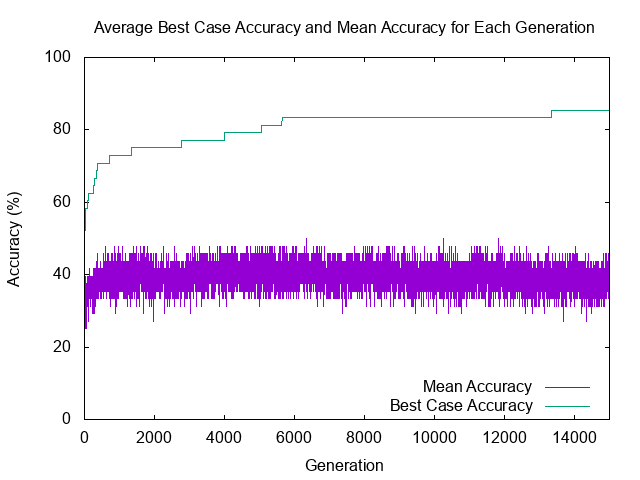
\includegraphics[width=\textwidth]{div_60.png}
		\caption{}
		\vspace{1em}
		\label{fig:div_6}
	\end{subfigure}
	~
	\begin{subfigure}[ht]{\textwidth}
		\centering
		\begin{tabular}{ccccc}
			\toprule
			& \bfseries{Diversity Weighting (\% of Accuracy)} &
			\bfseries{Perf. Runs (\%)} &
			\bfseries{Avg. Execution Time (s)} & \bfseries{Avg. Final Fitness}\\
			\midrule
			(a) & 0 & 16 & 235 & 40\\
			(b) & 20 & 23 & 238 & 44\\
			(c) & 40 & 13 & 231 & 42\\
			(d) & 60 & 10 & 247 & 41\\
			\bottomrule
		\end{tabular}
	\end{subfigure}

	\caption[Diversity weighting test results]{Diversity weighting test results;
	population size 50, elitism, tournament selection of size 20, probability
	of single point crossover 0.7, and a multi-objective fitness function with
	diversity weighting set to (a) 0\%, (b) 20\%, (c) 40\%, and (d) 60\% the weighting
	associated with accuracy.}
	\label{fig:div}
\end{figure}

\todo prune away graphs placed on the same page

Figure~\ref{fig:div} demonstrates the symptoms indicating existing on either side of
balance of power within the fitness fuction between accuracy and diversity. With a
weighting of 0 (Figure~\ref{fig:div_0}) the population hits two evolutionary dead ends,
one at accuracy 34, which it eventually manages to summount and another at accuracy 40
which it fails to improve beyond. The lack of diversity is also clear in the narrow
variance in mean population accuracy. On the other end of the spectrum a weighting of
60\% (Figure~\ref{fig:div_6}) achieved worse perfect solutions but was able to reach
an averge ending accuracy of 41, and all improvements to fitness occured relatively
regularly. This indicates a diverse population with only a small incentive to improve
their accuracy. Balancing this, and improving on the previous best, decreasing the
weighting from 40\% to 20\% seemed to better sit between the two extremes presented
by Figure~\ref{fig:div_0} and Figure~\ref{div_6}.

The reduced effectiveness of diversity at higher weightings is somewhat at odds with
the point of view presented by (\todo cite the multi-objective). As previously mentioned
however their implimentation was coupled with an effective pruning mechanism to dissuade
mindless diversification for the sake of diversification. Also the context each multi-objective
fitness function differs, evolutionary hardware and evolutionary programming are different
animals each with distinct problems. Namely (\todo cite) present theirs as a mechanism
for avoiding the run-away bloat that can happen with evolutionary programming where
the program needlessly gets longer, whereas here we are spacially capped at the size of
the FPGA, looking for a solution within it's confines. It is a subtle difference but
could explain the disparity in results.

\subsection{Coevolution}

Can we exchange the full problem testing system used thus far for a coevolved
parasite population of evolutionarily targeted problems? In order to answer that
question experiments emplying coevolution were conducted on the evolutionary
system developed thus far. Experiments were conducted with a parasite problem
size of 8, 16, and 32; and the best performing parameter choice was repeated
without elitism.

\todo Talk about all the coevolutionary problems from Bullocks paper

\begin{figure}
	\centering
	\begin{subfigure}[ht]{0.49\textwidth}
		%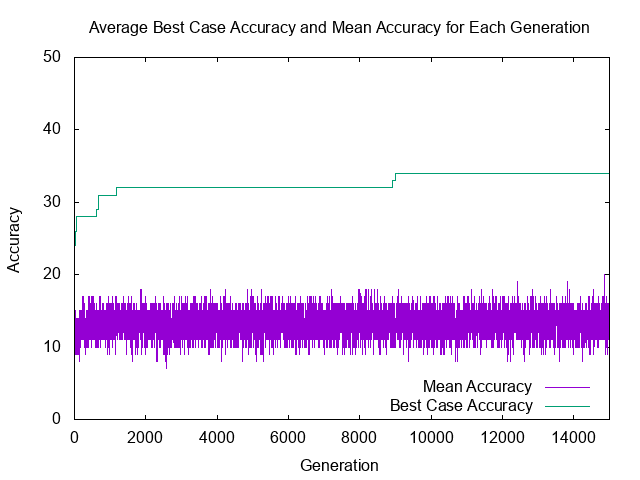
\includegraphics[width=\textwidth]{coev_8.png}
		\caption{}
		\vspace{1em}
	\end{subfigure}
	~
	\begin{subfigure}[ht]{0.49\textwidth}
		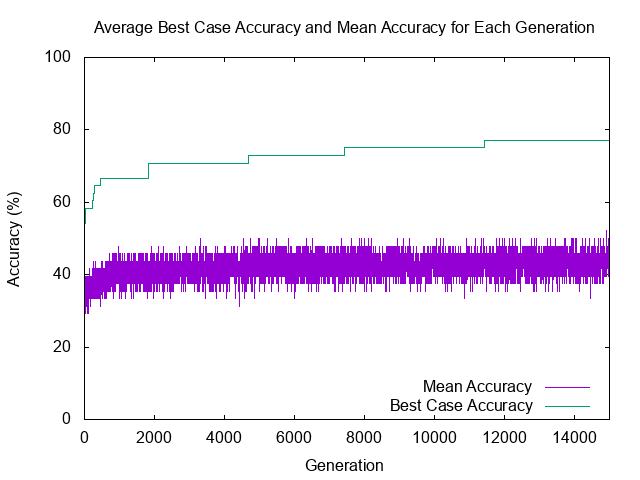
\includegraphics[width=\textwidth]{coev_16.png}
		\caption{}
		\label{fig:coev_16}
		\vspace{1em}
	\end{subfigure}
	~
	\begin{subfigure}[ht]{0.49\textwidth}
		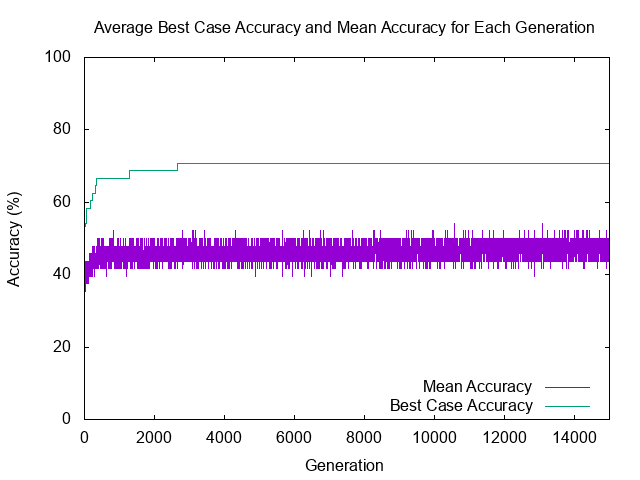
\includegraphics[width=\textwidth]{coev_32.png}
		\caption{}
		\vspace{1em}
	\end{subfigure}
	~
	\begin{subfigure}[ht]{0.49\textwidth}
		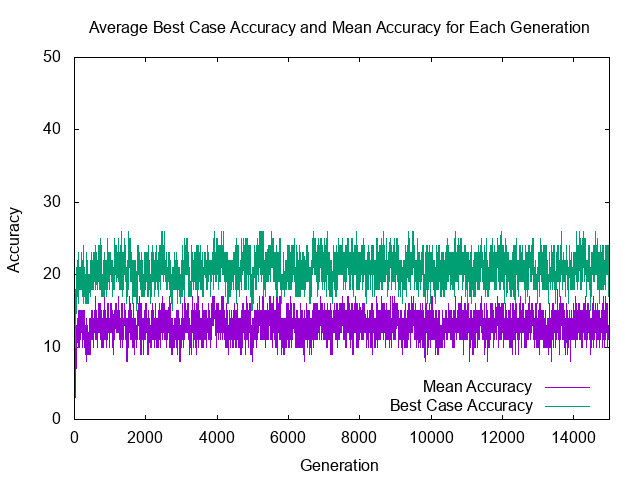
\includegraphics[width=\textwidth]{coev_no_elit.png}
		\caption{}
		\label{fig:coev_16_no_elit}
		\vspace{1em}
	\end{subfigure}
	~
	\begin{subfigure}[ht]{\textwidth}
		\centering
		\begin{tabular}{ccccc}
			\toprule
			& \bfseries{Parasite Size} &
			\bfseries{Perf. Runs (\%)} &
			\bfseries{Avg. Execution Time (s)} & \bfseries{Avg. Final Fitness}\\
			\midrule
			(a) & & & & \\
			(b) & 16 & 0 & 605 & 37 \\
			(c) & 32 & 0 & 703 & 34 \\
			(d) & 16 & 0 & 535 & 24 \\
			\bottomrule
		\end{tabular}
	\end{subfigure}

	\caption[Coevolution test results]{Coevolution test results;
	population size 50, elitism, tournament selection of size 20, probability
	of single point crossover 0.7, a multi-objective fitness function with
	diversity weighting set to 20\%, and a coevolved parasite population where
	each parasite is of size
	(a) 8, (b) 16, and (c) 32 tests. (d) has a parasite consisting of 16 tests
	but elitism is turned off.}
	\label{fig:coev}
\end{figure}

In a coevolutionary system there a series of problems that can disturb the gentle
ballance between host and parasite.
In Figure~\ref{fig:coev} no coevolutionary system was capable of evolving a successful
solution. Each had poor execution time and low final fitness.

Earlier in this document coevolution was touted as a potential solution to the scaling
problem, however comparing Figure~\ref{fig:coev_16} and Figure~\ref{fig:coev_16_no_elit}
it is clear that without elitism the entire system becomes unable to produce a solution
with even somewhat acceptable accuracy. This rehiterates the findings in subsection
~\ref{ss:elitism} in this new context. In order for elitism to have any real impact
with the binary addition problem members of the population have to be exhaustively tested
against all possible problems to allow the elitism metric to keep the best performing
individual regardless of the parasite they are paired against. This disrupts the
notion that coevolution can be used to aid with the scaling issue and will be further
discussed in Section~\ref{s:scaling}.

In all the experiments with elitism activated after
a certain amount of time the average population
fitness reaches a plateau and all improvements seem to come from the highest performing
individual(s) with little impact in the overall population. Although similar to
tests not using a coevolutionary system this behaviour could be indicative
of a disengaged population, one in which the parasite population becomes too aggresive
and becomes unbeatable, no longer discriminating in the host population between FPGA
configurations.

\todo Change the virulence

\subsection{Evolved 2-bit addition hardware}
By now we have a relatively well performing evolutionary hardware system,
tailored directly for the binary arithmatic problem. With this we can explore
a range of uses within the domain of dynamic problems.

Talk about all the cool stuff, success rate etc analyise the given circuit
beyond simple correctness. Diagram clearly one produced via crossover

\begin{figure}
	\centering
	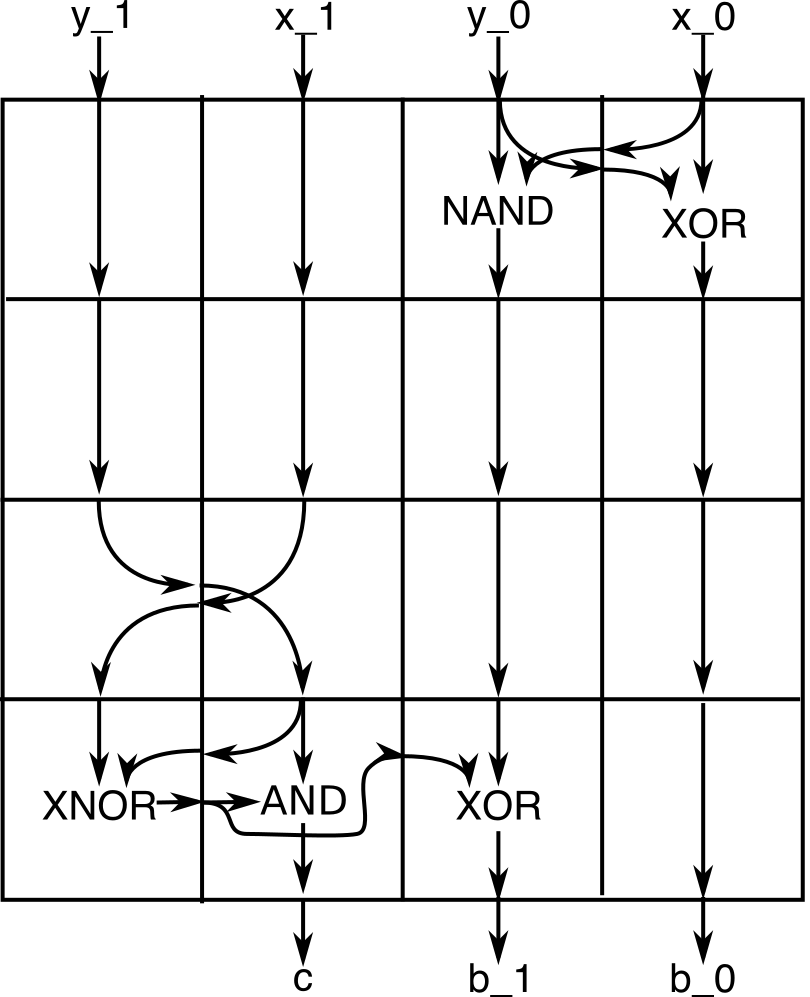
\includegraphics[width=0.45\textwidth]{evolved_adder.png}
	\caption{Successful 2-bit binary addition evolved hardware}
	\label{fig:2-bit}
\end{figure}

\section{Fault tollerance}

The dynamic problem with the largest immediate impact is arguably that of
a system experiencing faulty behaviour.
With a tuned genetic algorithm, exploration into the capacity to dyanmically
adapt the configuration in the face of such a changed or changing problem provides
the oportunity to thoroughly test fault recovery and mitigation strategies.

Using the fault simulation framework built into the FPGA simulation a series
of targeted or randomly generated faults will be introduced to an in-progress
genetic algorithm.

\subsection{Simple Fault Recovery}
By preloading the genetic algorithm with a hand designed 2-bit adder and then
simulating a highly targeted critical fault withing the function of a CLB insight
can be gained into the capcity of evolvable hardware to act as a fault recovery
system in itself and provide a reliable method of recalibration should a device
experience a fault which would otherwise render it useless.

\begin{figure}
	\centering
	\begin{subfigure}[ht]{0.45\textwidth}
		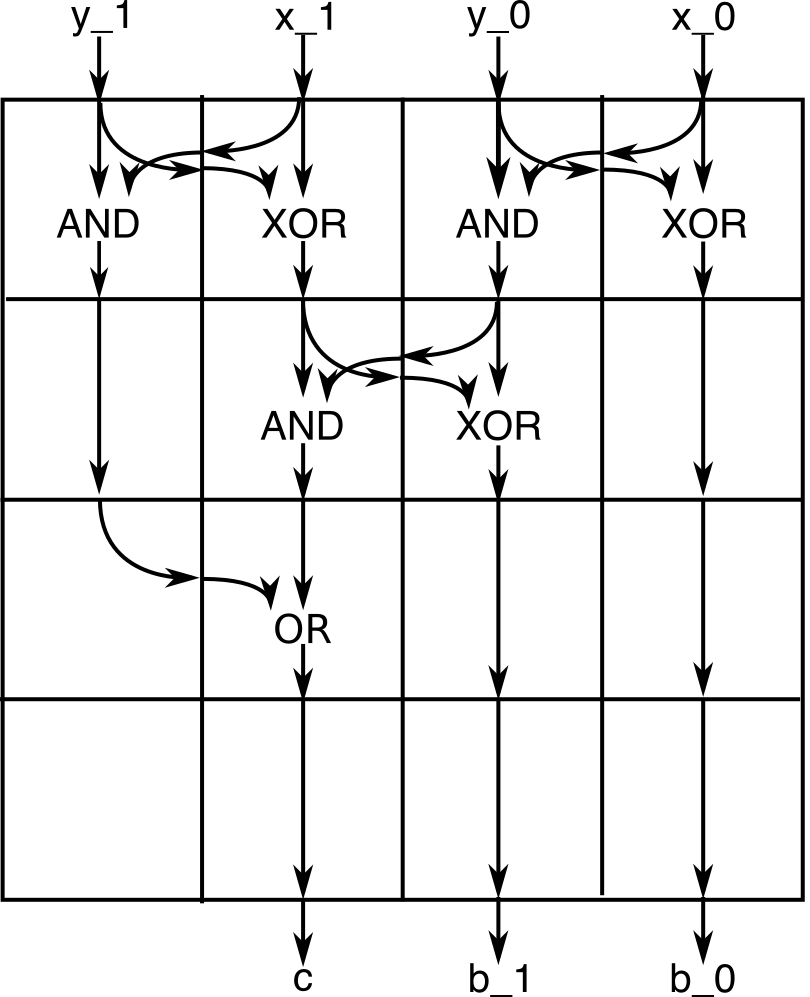
\includegraphics[width=\textwidth]{perfect_adder.png}
	\end{subfigure}
	~
	\begin{subfigure}[ht]{0.45\textwidth}
		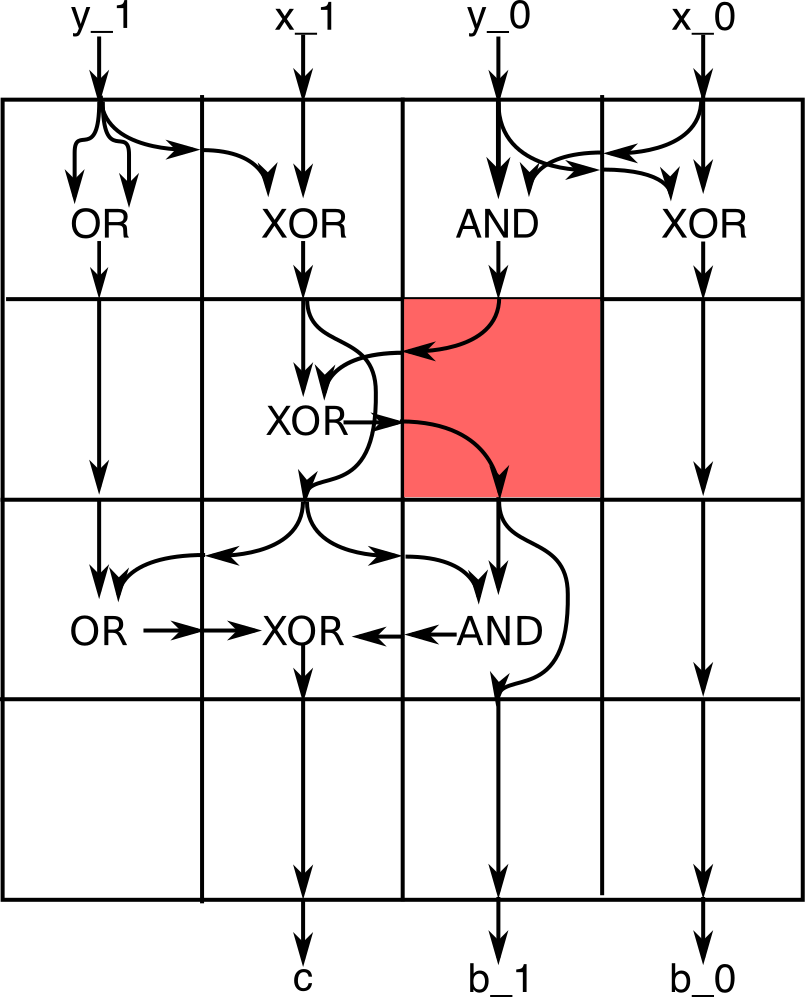
\includegraphics[width=\textwidth]{perfect_adder_fault.png}
	\end{subfigure}
	\caption{Fault recovery}
\end{figure}

\subsection{``Sticky" Fault Mitigation}
Evolutionary hardware can be used to recover from otherwise devastating faults. In the example below the outputs of the operation F within the CLB marked in red were clamped to a value representing an “undefined output”. Starting with the ideal configuration on the left and activating the fault, the genetic algorithm recognised the current solution as suboptimal and generated the configuration on the right.

Simulating a sticky fault by activating and deactivating a fault every 500 generations results in the fitness graph above on the right. When the fault is activated it has an adverse affect on fitness, but a solution is found which works when the fault is both active and inactive.

Sticky faults improve diversity and therefore improve training, maybe

Different from normal Fault tollerance - this is the sticky fault model to find a design okay for all, instead the evolution happens when the fault is detected to recover

\section{Dynamic problem optimisation}
By introducing subtraction as a problem alongside addition, the relative weightings of a correct answer for each problem can be varied to explore dynamically changing problems. In the graph below the genetic algorithm starts with a perfect ADDer and 100\% of the fitness weighting assigned to correct ADDs, every 200 generations this shifts by 10\% towards SUBs.

\section{Scaling \label{s:scaling}}
In an effort to improve how an evolvable hardware system scales observing
how the dynamics of a coevolutionary system vary as the number of parasites
fluctuates could indicate a potential mechanism to reduce the number of
test cases required per evaluation and therefore improve evaluation time.

Evaluating the execution time and correctness of the solutions generated
by the genetic algorithm as we reduce the size of the parasite should
quantify the feesability of this idea.

Scafolding vs non-scafolding, coevolution to improve scalability of finess evaulation (tests grow expontentiallly as input bits increase)

Table of timings
\begin{figure}
	\centering
\begin{tabular}{ccc}
	\toprule
	\bfseries{FPGA Size (Width x Height)} & \bfseries{Full test} & \bfseries{Coevolve (Size 16)}\\
	\midrule
	2x4 & & \\
	4x4 & 238 & 535\\
	6x4 & & \\
	8x4 & & \\
	\bottomrule
\end{tabular}
\caption{Execution time (s) for genetic algorithm opperating on different FPGA sizes with
a full evaluation or a coevolved parasite population (without elitism).}
\end{figure}

The trouble with using coevolition to improve scaling is to stop elitism
every individual has to be tested against the whole suite of problems, and
without elitism the entire system breaks down. A high mutation rate is required
to effectivly persue the solution. Really bloody bad lol.

\section{Evolution good}
better than bruteforce
mention things set out to do and address challenges

\section{Evolution bad}
Intermittent leap from primordeal soup



% -----------------------------------------------------------------------------

\chapter{Conclusion}
\label{chap:conclusion}

{\bf \color{red}A compulsory chapter,     of roughly $5$ pages} 
\vspace{1cm} 
\section{Summary of Achievements}
My intention of recreating the genetic algorithm from Thompson's work on
evolutionary hardware \cite{10.1007/3-540-63173-9_61} and applying it to the
binary arithmetic problem was successful, as outlined in Chapter~\ref{chap:evaluation}.
The initial genetic algorithm parameters in Section~\ref{s:ga_tune} mirror
Thompson's exactly. When applied to 2-bit binary addition the algorithm
executed quickly but in 30 repeated executions to generation 15000, failed to produce a perfect
binary ADDer. The average final accuracy was 40 over 30 runs, out of a maximum of 48.

This baseline algorithm was then improved on by factoring in features from
modern genetic algorithm and evolvable hardware literature.
These features included; a
multi-objective fitness function incorporating a diversity measurement,
mutation rate variation, tournament selection, varied crossover probability,
the absence of elitism, population size, multi-objective weightings, and
coevolution (with varied virulence). Assessing each of these in turn
a 2-bit binary addition specific genetic algorithm was devised with vastly
improved performance. In repeated experiments almost 1/4 of executions to
generation 15000 produced a perfect solution will 100\% accuracy. This
executed in comparable time to the initial parameters specified in
\cite{10.1007/3-540-63173-9_61}, and achieved an average final fitness of 44,
a clear improvement. Using a t-test this was shown to be a statistically significant
improvement.
The search space of FPGAs defined by 32 byte strings is huge. Clearly the
scheme devised in this dissertation is a vast improvement over enumerated bruteforce
search.

This system was then exposed to a series of dynamic problems; simple fault
recovery, ``sticky" fault mitigation, and shifting weighting optimisation.
The system coped admirably with simple fault recovery; when a critical fault
was injected in the FPGA simulation the accuracy dropped to a crippling low.
In repeated executions, by 14000 generations evolving with the fault 43\%
had developed perfect solutions, and the average accuracy was 42. The success
rate here is incredibly high when compared to the performance of the underlying
evolvable hardware system which achieved perfect answers on 23\% of repeated executions.
With a single oscillating ``sticky" fault on 7\% the genetic algorithm was
able to devise a solution which worked both in the presence of the fault and without
it. Even with two faults clear improvements in how the system coped with shifting
correctness criteria are visible.

The entire evolvable platform is available on GitHub. The FPGA simulation
is a distinct component which exposes concise functionality to the evolutionary
software component. The simulation can be downloaded independently and used
not only as a component in other evolutionary systems but in any software project
which could make use of a streamlined generic FPGA simulation of arbitrary developer
defined size. The usefulness of the ability to convert binary strings into FPGAs and evaluate specified
configurations extends beyond the context presented here and could form the backbone
of a plethora of speculative hardware projects. This fits the FPGA simulation
specification outlined in the project aims.

Exploration into the scaling problems of evolvable hardware outlined the key
offenders contributing to extreme execution times. With simulated hardware
the execution time scaled nicely with FPGA size, but the clear culprit in
slow evaluation cycles was the sheer number of trails conducted for larger
problems. Coevolution was proposed as a mitigation strategy, and would reduce
the number of trials conducted; however, performance under the 2-bit problem
was severely disappointing and was completely unsuitable as a replacement to
conventional exhaustive testing. In order to achieve any sort of success
elitism was non-optional and this required uniform exhaustive testing to function
properly. Even without the extra computation required for elitism, the overheads
maintaining a second distinct evolutionary population lead to extreme average
execution times.

A GUI was developed to provide visual feedback on the population health
and genetic algorithm performance in an attempt to improve user understanding
of the underlying process and drive parameter choices. This was somewhat successful,
but the vast quantity of information on hand had to be reduced; the only detailed
information on offer was for the current generation's best performing individual.
For this an exhaustive list of test performance and a diagram of the FPGA configuration
was provided to the user. The remaining population qualities were reduced to a handful
of statistics; generation number, mean accuracy, and mean diversity. More innovation
is required in this domain to truly offer a way to monitor a population and guide
parameter choice.

There are a great number of limitations existing within this project, and
evolvable hardware in a wider sense. 2-bit addition to most would seem trivial,
and even though the execution time was painlessly short, directly extending
this to 3-bit addition required 1473s and 4-bit addition 8537s. Designing an
iterative design system around any larger problem than 2-bit binary arithmetic
is simply not an option. Extending
any assumptions here to useful applications requires solving a great number of
challenges.

Visual inspection of many of the accuracy graphs in Chapter~\ref{chap:evaluation}
could lead a reader to believe that many improvements are simply lucky leaps from
a general background population which usually performs moderately; and the reader
would not be wrong. Population quality tends to reach a certain value and then
remain consistent, and best-case improvements become fewer and far between as
execution continues. The only way a system is saved from backtracking is by the
including of an elitism mechanic. These together indicate that the population improves
until a certain value and then maintains a primordial soup, rarely performing well
but on occasion generating an example with an improved performance. The cycle repeats
but making improvements requires larger and larger leaps from this primordial soup.

The disparity between vanilla evolutionary hardware in Figure~\ref{fig:div_2}, only
achieving a success rate of 23\% and the fault injection examples in
Figure~\ref{fig:simple_fault} achieving 43\% highlights the tendency for
this evolvable hardware incarnation to stumble blindly into evolutionary dead ends,
often dwelling needlessly on bloated hopeless solutions. These solutions take up
too many of the resources allotted to the FPGA to achieve their mostly-good results
to progress to perfection.

The system optimisation under dynamically shifting weightings is underwhelming,
until the system is placed under real pressure the evolutionary tactic seems to be
to maintain the current solution rather than perform minute tweaks to gain a performance
advantage. The domain specific knowledge required to design hardware, through
evolvable hardware, is replaced by domain specific knowledge for genetic algorithm
design.

\section{Project state}
A fully flexible binary arithmetic evolutionary hardware platform works, with
a plethora of options and configurable components. The FPGA simulator and GUI are a distinct
self contained entity allowing for use in machine learning hardware design beyond
genetic algorithms.

\section{Further work}
Given the self contained nature of the underlying FPGA simulation there is scope to
extend this project with more machine learning mechanism to optimise the FPGA
configuration for the binary addition problem. Further study into the underlying
structure of the search space could provide insights which would allow further
tuning of the genetic algorithm or, more likely, open the door to more esoteric
specific implementations of other techniques, such as neural networks.

Remaining close to genetic algorithms the nature of the mutation function
could shift. Rather than comprising random bitflips there could be a chance
of a predefined operation with knowledge of the phenotype to genotype mapping,
such as; cell translation/rotation, cell reordering, or mirroring cell connections.
Such a modification would move this exploration to the fringes of genetic algorithm
research, if not beyond the realm of, as genetic algorithms conventionally do not
have any in-build understanding of what the genetic material represents (beyond the
evaluation step).

If the plethora of issues surrounding system scaling could be addressed
one could conceive of a hardware system similar to what was proposed in
\cite{10.1007/3-540-61093-6_6}, save for a general purpose processor.
Specific fault-prone units could be replaced with micro-FPGAs, each preloaded
with the original component specification. Upon the detection of a fault
the genetic algorithm begins. This iterates over the design finding ways to
capitalise on the demonstrated fault recovery performance and devise a unit
which works perfectly in the presence of the fault. The vast majority of modern systems are multi-core
so it is not unthinkable that should a component in one core fail any alternative
cores could initiate and conduct the self-healing process. These systems
could take advantage of evolvable hardware accelerator chips to create
truly rugged circuitry. The evolutionary search could be conducted in
CPU idling time, and even if it takes hours, a component which wouldn't
otherwise work could be operational; ideal for satellites and/or operations
working on a scale such that brief component downtime for the sake of
longevity is not a huge issue.

If improvements in algorithm design leads to an evolvable hardware system
which, when confronted by a dynamically shifting weighted problem, can
perform prompt adjustments (at a speed faster than presented in this document)
then a flexible pseudo-FPGA-CPU as outlined above could facilitate
user/program specific fine tuning. Given contextual information (which shifts
the desirability of certain functions and therefore the weightings) the
processor could recalibrate to better suit it's function. Suppose,
as a trivial example, user A performs a great deal of multiplication,
and user B loves subtraction; given this information the processor should
be able to optimise for each. Rather than trying to be accurate the processor
could be assumed to be constantly accurate (other wise it will not change)
and is instead trying to optimise for execution time.
performs a lot of multiplication


% =============================================================================

% Finally, after the main matter, the back matter is specified.  This is
% typically populated with just the bibliography.  LaTeX deals with these
% in one of two ways, namely
%
% - inline, which roughly means the author specifies entries using the 
%   \bibitem macro and typesets them manually, or
% - using BiBTeX, which means entries are contained in a separate file
%   (which is essentially a databased) then inported; this is the 
%   approach used below, with the databased being dissertation.bib.
%
% Either way, the each entry has a key (or identifier) which can be used
% in the main matter to cite it, e.g., \cite{X}, \cite[Chapter 2}{Y}.

\backmatter

\bibliography{dissertation}

% -----------------------------------------------------------------------------

% The dissertation concludes with a set of (optional) appendicies; these are 
% the same as chapters in a sense, but once signaled as being appendicies via
% the associated macro, LaTeX manages them appropriatly.

\appendix

\chapter{simulator.h}
This shows the functionality exposed to the evolvutionary front-end by the
FPGA simulator, and how internal data is organised.

\begin{lstlisting}
#include <stdio.h>
#include <ncurses.h>
#include <curses.h>
#include <math.h>

#define FPGA_HEIGHT 4
#define FPGA_WIDTH 4
#define STRING_LENGTH_BYTES FPGA_WIDTH * FPGA_HEIGHT * 2
#define FAULT_NUM 0
#define FAULT_TYPE_CON 0

typedef enum {
	OFF,
	NOT,
	OR,
	AND,
	NAND,
	NOR,
	XOR,
	XNOR
} Gate;

typedef enum {
	NORTH,
	EAST,
	SOUTH,
	WEST,
	F
} Direction;

typedef struct {
	int x, y;
	Direction dir;
	unsigned char value;
} Fault;

typedef struct {
	Direction n_out, e_out, s_out, w_out;
	Gate gate;
	Direction g_in1, g_in2;

	//3 values: 0, 1, 2 (2 represents undefined)
	unsigned char n_in, e_in, s_in, w_in;
	unsigned char n_val, e_val, s_val, w_val;
} Cell;

typedef struct {
	Cell cells[ FPGA_HEIGHT ][ FPGA_WIDTH ];
	unsigned char control;
	unsigned char input[ FPGA_WIDTH ];

	Fault faults[ FAULT_NUM ];
	int active_fault[ FAULT_NUM ];
} FPGA;

/*
 * FPGA is defined by a bitstring of the following format:
 * 		- the bitstring defines cells from left to right, top to bottom, row by row, one byte per cell
 * 		- the least significant 2 bits define the value pushed to n_out (F,EAST,SOUTH,WEST)
 * 		- the next 2 define the value pushed to e_out (NORTH,F,SOUTH,WEST)
 * 		- the next 2 define the value pushed to s_out (NORTH,EAST,F,WEST)
 * 		- the next 2 define the value pushed to w_out (NORTH,EAST,SOUTH,F)
 * 		- the next 2 define where the first input for F comes from (NORTH,EAST,SOUTH,WEST)
 * 		- the next 2 define where the second input for F comes from (NORTH,EAST,SOUTH,WEST)
 * 		- the next 3 define the function F performs (OFF,NOT,OR,AND,NAND,NOR,XOR,XNOR)
 * 		- the most significant bit is reserved
 */

void bitstring_to_fpga ( FPGA *fpga, unsigned char *bits );

void evaluate_fpga ( FPGA *fpga );

void init_curses ();

void redraw ( int iteration, FPGA fpga, int most_fit, int mean_fit, int mean_div, int add_weight, int sub_weight );

void tidy_up_curses();
\end{lstlisting}

\label{appx:sim}

\chapter{evolve.h}
\label{appx:evolve}
\begin{lstlisting}
#include <stdio.h>
#include <stdlib.h>
#include <time.h>
#include <fcntl.h>
#include <unistd.h>
#include <math.h>
#include "simulator.h"

#define POP_SIZE 400
#define MUTATION 0.5f
#define SIZE_WEIGHT 0
#define DIVERSITY_WEIGHT 4
#define ELITISM 1
#define FITNESS_WEIGHT 10
#define COEVOLVE 0
#define STICKY 0
#define LOG 1
#define PROB_SKEW 0.0f //between 0 or 1, 1 is linear
#define VIRULENCE 1.0f
#define PARASITE_SIZE 16

int add_weight, sub_weight;

typedef struct Individual {
	unsigned char values[ STRING_LENGTH_BYTES ];
	int eval[ 3 ];
	FPGA fpga;
} Individual;

typedef struct Parasite {
	unsigned char values[ PARASITE_SIZE ];
	float score;
} Parasite;
\end{lstlisting}

\chapter{Experimental Results}
\label{appx:evolve}
\todo some meaty tables here

% =============================================================================

\end{document}
